%%%%%%%%%%%%%%%%%%%%%%%%%%%%%%%%%%%%%%%%%
% Diaz Essay
% LaTeX Template
% Version 2.0 (13/1/19)
%
% This template originates from:
% http://www.LaTeXTemplates.com
%
% Authors:
% Vel (vel@LaTeXTemplates.com)
% Nicolas Diaz (nsdiaz@uc.cl)
%
% License:
% CC BY-NC-SA 3.0 (http://creativecommons.org/licenses/by-nc-sa/3.0/)
%
%%%%%%%%%%%%%%%%%%%%%%%%%%%%%%%%%%%%%%%%%

%----------------------------------------------------------------------------------------
%	PACKAGES AND OTHER DOCUMENT CONFIGURATIONS
%----------------------------------------------------------------------------------------

\documentclass[12pt]{diazessay} % Font size (can be 10pt, 11pt or 12pt)

%----------------------------------------------------------------------------------------
%	TITLE SECTION
%----------------------------------------------------------------------------------------

\title{\textbf{Course: Física Teórica I (CDP7600)} \\[0.2cm] {\Large \textbf{Project}: \hspace{0.2cm}
\textit{Fibration building blocks of information-processing networks}
}}% Title and subtitle

\author{\textbf{Higor da S. Monteiro} \\ \textit{Universidade Federal do Ceará}} % Author and institution

\date{\today} % Date, use \date{} for no date

%----------------------------------------------------------------------------------------

\begin{document}

%\maketitle % Print the title section

\begin{center}	
	{\LARGE \textbf{Project Report: Física Teórica I}}\\[0.25cm]
	{ $\bullet$ }\\
	\vspace{0.25cm}
	{\large \textbf{Identification and classification of information-processing building blocks on genetic regulatory network}}\\[0.25cm]
	{ Higor da S. Monteiro }\\
	{ $\bullet$ }\\
	{ Departament of Physics - Universidade Federal do Ceará(UFC) }\\
	{ Fortaleza, Ceará }\\
	{ November, 05, 2019 }\\[0.75cm]
	{\textbf{Abstract}}
	
\end{center}

Fibration building blocks of information-processing networks represent the sets of nodes that are symmetrical with respect to the processing of input signals received from the rest of the network, defining this way the classes of nodes that process equivalent information. In this report, I reproduced relevant results concerning the identification and classification of the fibration building blocks of directed networks, constructed from real systems data. More specifically, using the transcriptional regulatory network data from the \textit{Escherichia Coli} bacteria, I quantify the clusters of nodes in the network that synchronously process equivalent information, and then I classify these clusters, called fibers, based on its specific topological features. Here, to present the obtained results, I briefly introduce the theory concerning the graph fibration morphism and its main definitions related to information processing symmetries. Then, I detail the computational methods adopted to the identification of the network fibers, presenting the algorithmic approach for the problem in hand, based on the general relational refinement partitioning algorithms described by Paige and Tarjan in 1987. After defining the implementation details of the graph refinement algorithm I apply the method for trial network examples and then for the constructed genetic regulatory network of \textit{Escherichia Coli}, noticing the equivalence between the results obtained by the methods described in this report and the results exhibited in the most recent literature given at \textit{Morone et. al.} (2019). The results showed in this report, concerning the fibers distribution over the network, are tested and verified to support the assertion that the algorithm used captures the correct minimal fibration.

%----------------------------------------------------------------------------------------
%	ABSTRACT AND KEYWORDS
%----------------------------------------------------------------------------------------

%\renewcommand{\abstractname}{Summary} % Uncomment to change the name of the abstract to something else


\vspace{30pt} % Vertical whitespace between the abstract and first section

%----------------------------------------------------------------------------------------
%	ESSAY BODY
%----------------------------------------------------------------------------------------

\section{Introduction}

Dynamical processes occurring in networks permit novel qualitative behaviors that are not directly measured in classical dynamical systems \cite{Stewart2006}. The main feature of these behaviors is the existence of verifiable partial synchronized states, where different elements in the system follow the same or correlated phase space trajectories. These synchronized states are fundamentally important for the study of dynamical phenomena in networks, being still more relevant for information-processing complex systems, in which synchrony is directly related to functionality.

Besides the specific characteristics of the dynamics taking place on the network, it is possible to define states of partial synchrony by considering only the topological features of networks. To this, it is possible to define a natural graph partitioning where each element of it represents the set of nodes that process equivalent incoming information from the rest of the network and even from itself, implying that each of these nodes processes information synchronously.  Furthermore, one of the important insights concerning these clusters of synchronized network elements is the direct association of symmetries groups with the resulted distribution of synchronization clusters, which can offer a precise procedure to identify and classify the information-processing building blocks of several networks in nature.

However, recently some works has been recognizing that topological symmetries of the network structure, meaning neighborhood structure invariance under nodes permutation, are not actually necessary for the emergence of synchronization of node states. Thus, instead of very restrictive isomorphisms rules, the blocks of synchronized information processing obeys a more loose concept of symmetry represented by the rules of groupoids. More specifically, information flow in a directed network is maintaneid as invariant under a graph fibration morphism. A graph fibration is a transformation that keeps invariant the set of universal input-trees that group the network nodes into functional blocks called network fibers \cite{Boldi2006}, \cite{fibration2019}.

The formal definition of an input-tree is explained in detail at \cite{fibration2019}, \cite{Boldi2006} and \cite{Boldi2002}. Here, I give just a direct and intuitive example through the examples showed at figures \ref{fig:ex}. To fully characterize the information flow directions in a directed network, we can define for each node in the network an input-tree containing all the information pathways that ends at the given node. Thus, if two different nodes have isomorphic input-trees, which means that they receives equivalent information from the network, they synchronize their dynamical states, exhibiting a correlated behavior for the network. Even more, if a group of nodes have isomorphic input-trees, then a graph fibration transformation reduces these nodes from network $G$ in one single node for a base network $G'$. This way, a fibration reduces the original network in a base network where each node of $G'$ represents a fiber block of $G$. In figure \ref{fig:ex} we can see a directed network formed just by three nodes. For each one, they differs only by the patterns of directed links, from which information can flow.
\begin{figure}[h]
	\centering
	\subfloat[]{{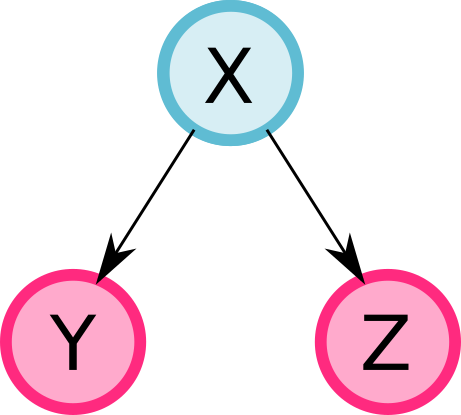
\includegraphics[scale=0.4]{Figures/ex1.png}}}
	\qquad
	\subfloat[]{{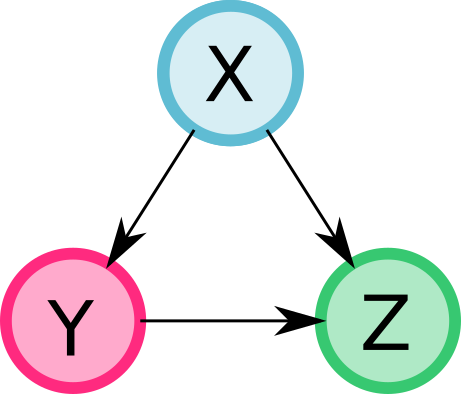
\includegraphics[scale=0.4]{Figures/ex2.png}}}
	\qquad
	\subfloat[]{{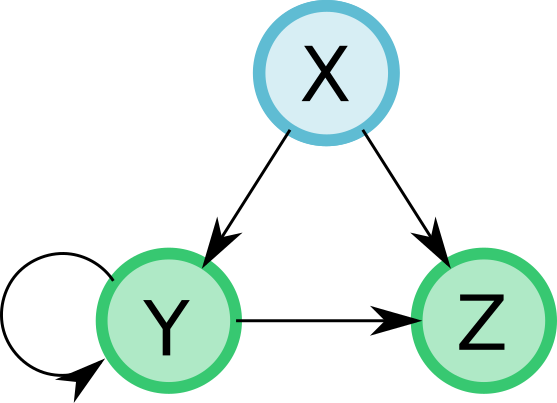
\includegraphics[scale=0.4]{Figures/ex3.png}}}
	\caption{First trial network example. Containing a total of $N = 17$ nodes and $M = 22$ arcs, the network has two weakly connected components, defined as the connected networks when we treat all the directed arcs as undirected edges. For each non-trivial fiber I give the same color for the nodes belonging to it.}
	\label{fig:ex}
\end{figure}

As we can see in figure \ref{fig:ex}, in the first case both $Y$ and $Z$ receives information only from $X$, for which it is obvious that $Y$ and $Z$ process the same information and then the two nodes synchronize their states (again not considering the details of the dynamics). However, if we allow that $Y$ sends information to $Z$ along with $X$, then $Z$ do not process the same information than $Y$, since it receives information from $X$ and $Y$, while $Y$ receives only from $X$ (\ref{fig:ex}b). To get around this inconvenience, we can simply add an autorregulation loop for node $Y$, allowing that $Y$ and $Z$ synchronize again (\ref{fig:ex}c).

All this discussion can be put on solid ground by considering the isomorphic relations between the input-trees of each node in the network. It is possible to note in figure (\ref{fig:inputex}a) and (\ref{fig:inputex}c) that the nodes $Y$ and $Z$ have isomorphic input-trees, which imply that the two nodes have synchronized states. Important to mention that because the addition of the autorregulation loop in the node $Y$, the input-tree that includes this loop becomes of infinite height, meaning the information loop flow in this directed link.

\begin{figure}[h]
	\centering
	\subfloat[]{{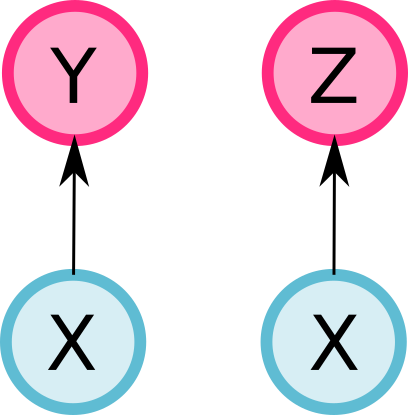
\includegraphics[scale=0.32]{Figures/ex1input.png}}}
	\qquad
	\subfloat[]{{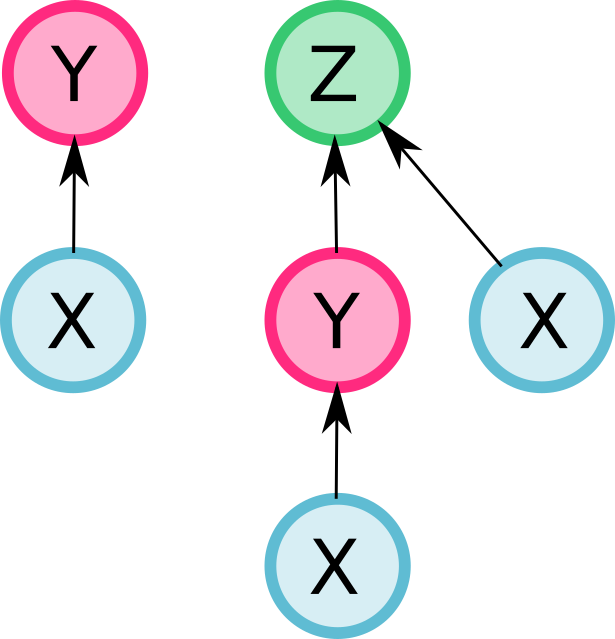
\includegraphics[scale=0.32]{Figures/ex2input.png}}}
	\qquad
	\subfloat[]{{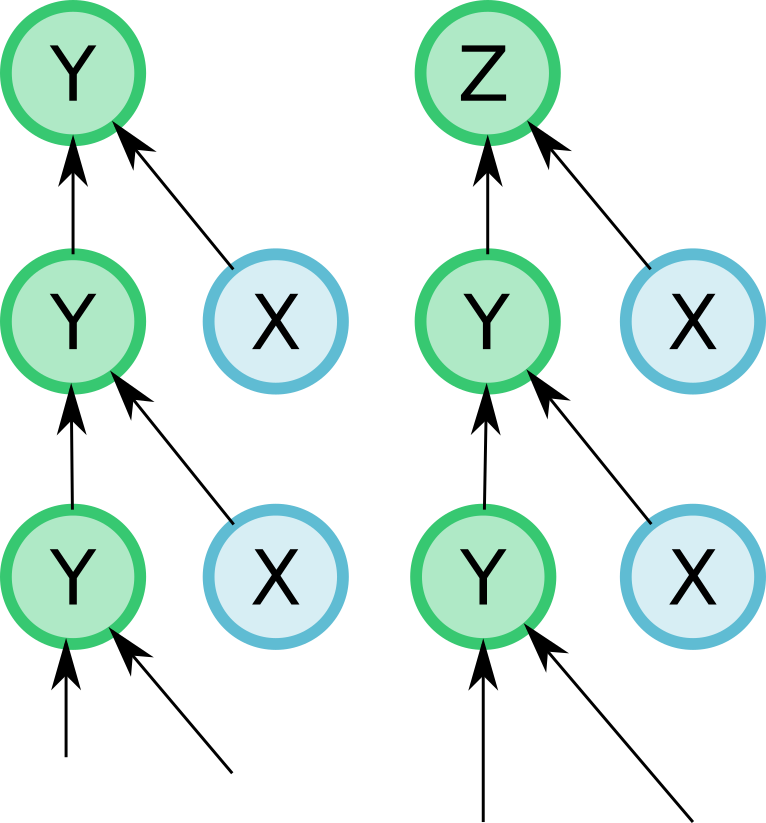
\includegraphics[scale=0.32]{Figures/ex3input.png}}}
	\caption{First trial network example. Containing a total of $N = 17$ nodes and $M = 22$ arcs, the network has two weakly connected components, defined as the connected networks when we treat all the directed arcs as undirected edges. For each non-trivial fiber I give the same color for the nodes belonging to it.}
	\label{fig:inputex}
\end{figure}

In practice, to identify if two nodes belongs to the same network fiber, \textit{i. e.}, if two nodes have isomorphic input-trees is only necessary to check the first-layer of their input-tree, called input-set \cite{norris1995}, which means that if two nodes belong to the same fiber block they have the same number of incoming links from the same fibers nodes. That implies that is not necessary that incoming neighbors be the same nodes, being only necessary that the incoming fibers are the same. 

At last, the identification of network fibration building blocks on biological regulatory networks is important because it allows the recognition of their information-processing building blocks, which is essential for the understanding of the functionalities intrisic to these regulatory network \cite{transistor2019}. Moreover, this approach can offer a persistent procedure to the study of biological function in networks comparing with methods based on statistical significance of common occurring subnetworks, like the one presented by the network motifs \cite{motifs2002}. The computational approach for a proper identification and classification of fibers in directed networks are explained below.

%------------------------------------------------

\section{\textit{Coarsest Refinement Partitioning }Algorithm}

To identify the correct distribution of fibers over the network it is necessary to define an efficient procedure to split the nodes into different disjoint partitions, from which all nodes inside the same partition must receive equivalent information from all other partitions. To do that, we treat our problem as the same as finding the coarsest relational refinement partitioning of a set of elements that have a binary relation between them. Since a network is completely defined by a set of node elements and a set of edges that comprehend all the binary relations, this approach can be used. Therefore, in this section, I detail the optimal algorithm used to find this coarsest partitioning in the context of graph fibrations and show the relatively simple implementation of this method.

The algorithm used in this project is a slightly modified version of the algorithm presented by Paige and Tarjan \cite{Tarjan1987}, \ having a runtime complexity of $\mathcal{O}(M\log N)$, where $M$ and $N$ are, respectively, the number of edges and nodes in the network, being almost linear with the size of the network. It is important to note that this algorithm has the same runtime order than the algorithm from Cardon and Crushemore \cite{Cardon1982}, in which the algorithm of minimal fibration from \cite{fibration2019} is based. However, the algorithm presented by Paige and Tarjan has a simpler implementation and smaller prefactors, exhibiting a better approach to our problem. Even though the algorithm has wider general applications, here I give the details of the algorithm implementation to the application for a network, so that I introduce the necessary definitions within this context.

\subsection{Algorithm description}

A network $G(V, E)$ is completely defined by the sets of the nodes elements $V$ and the set of the arcs $E$. The network has $N = |V|$ nodes that can have connections with one another defined by the set $E$, which contains $M = |E|$ ordered pair of nodes, denoting the directed links between the network nodes. Considering a network, we can define a graph partition $\bar{P}$ over $V$ as a set of pairwise disjoints subsets of $V$ whose union is all $V$, that is
\begin{equation}
	\bar{P} = \bigcup_{i} P_i
\end{equation}
where $P_i$ are the elements of the partition $\bar{P}$, called blocks. If we take an additional graph partition $\bar{Q}$ that has the property that all of its blocks are contained in a block of $\bar{P}$, we say that $\bar{Q}$ is a refinement partition of $\bar{P}$. Moreover, for a block $B \in \bar{P}$, we say that the block $B$ is stable with respect a set $S$ if either all elements of $B$ connects with an element of $S$ or none element of $B$ points to any element of $S$.

The stable partition concept is central to the problem of relational coarsest refinement partitioning and can be easily extended to graph problems, where the coarsest graph partition problem is that of finding, for a given set of directed links $E$ and an initial partition $\bar{P}$ over $V$, the coarsest stable refinement partition of $\bar{P}$, \textit{i. e.}, the minimal number of disjoint blocks subsets of $V$ that forms a stable refinement of $\bar{P}$. 

Considering the stability of partitions, for a proper identification of the network fibers as defined in the above section we ought to construct a stable graph partition that is equivalent to the coarsest refinement of the network (minimal number of blocks) with respect to the information processing of each node. For that goal, we need to extend the concept of stability over partitions for the case that accounts for the information processed by each block of the partition. Therefore, to identify the group of nodes with isomorphic input-tree, we require that the partition should be not only stable but \textbf{input-tree stable}. That means that for a subset $S \subseteq$ $V$, a graph partition $\bar{P}$ over the network $G(V, E)$ is input-tree stable with respect to $S$ if for all the block $B \in \bar{P}$, the following equality is satisfied for all the elements $x$, $y \in B$:
\begin{equation}
	| E^{-1}(\{x\}) \cap S | = | E^{-1}(\{y\}) \cap S |
\end{equation}
where $E(\{x\})$ and $E^{-1}(\{x\})$ represents, respectively, the set of nodes that directly receives information from $x$, and the set of nodes that sends information, via a directed link, to $x$. 

This way, we can benefit from the stability properties \cite{Tarjan1987} to construct a refinement algorithm step that can achieve, through a finite number of steps, a input-tree stable partition from an initial unstable partitioning of the network. This way, given a subset $S \subseteq V$, the refinement step has the effect to refine the current partition, input-tree unstable with respect to $S$, by replacing it for a new partition, now input-tree stable for $S$. With that objective, we define a split function \textit{I-split($S$, $\bar{P}$)} that receive as input the current partition and a set $S$ and returns as output a new input-tree stable partition with respect to $S$. Favorably, that function benefits from two major properties of stability (and input-tree stability): the stability inheritance by refinement and by union of sets. By reason of this refinement inheritance, a given set $S$ can be used only once by the function \textit{I-split}, guaranting that the partition, after all other refinement steps, will maintain as stable with respect to $S$. Moreover, since stability is inherited under union of sets $S$, after sets are used in \textit{I-split}, their union cannot be used for the function. Considering all these properties, the essence of the refinement algorithm can be stated as

\begin{quotation}
	\textbf{Refinement Algorithm}: Find a set $S$ in which the current partition $\bar{P}$ is input-tree unstable. Replace $\bar{P}$ by the output of \textit{I-split($S$,$\bar{P}$)}. Guarantees that the set $S$ or unions of used sets never be used again.
\end{quotation}

Since the finest partitioning possible is the one in which every node is itself a block, the refinement step may be proceeded at most $N-1$ times, guaranting that the algorithm terminates with the correct answer, since stability is inherited by the refinement process. However, to guarantee that the algorithm has an optimal runtime we have to find a efficient way to select the appropriate sets to the refinement step, without choosing repeated ones. Fortunately, this can be easily done for the construction of a input-tree stable partition.

Given a set $S$ of nodes from the network $G(V, E)$ and a given input-tree unstable graph partition $\bar{P}$, the blocks $B \in \bar{P}$ that are input-tree unstable with respect to $S$ can be splitted into several blocks $B_j$ that will be stable input-tree with respect to $S$. Then, each splitted block will have the property defined by
\begin{equation}
	B_j = \{ x \in B : | E^{-1}(\{x\}) \cap S | = j \}
\end{equation}
where the number of splitted block must be larger than one to a proper splitting process take place. Then, for each unstable block $B \in \bar{P}$, all the splitted block, except the largest one, can be put at the back of a queue to be used ahead in the algorithm as a refinement set. This ensures that none repeated sets or union of repeated sets can be used during the algorithm execution.

\begin{figure}[t]
	\centering
	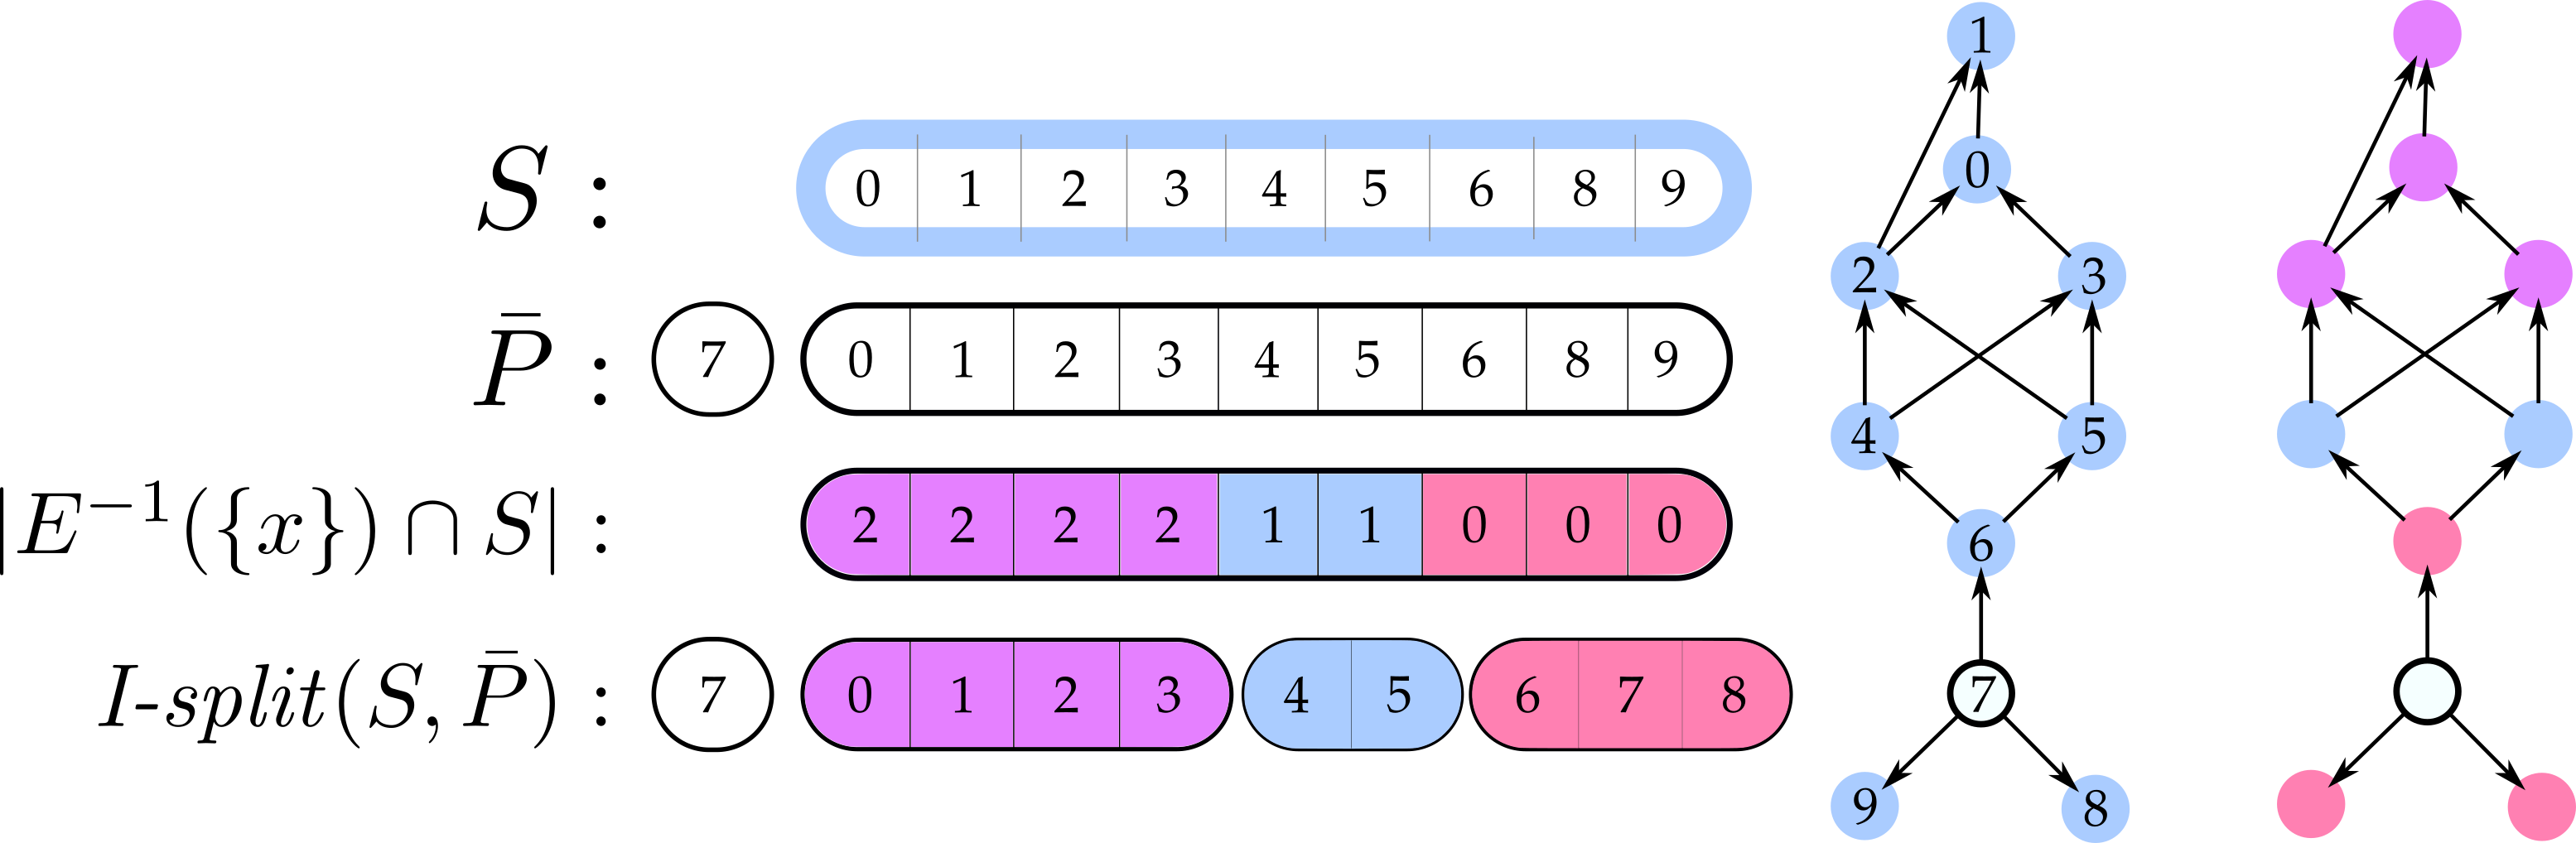
\includegraphics[scale=0.28]{Figures/split-function.png}
	\caption{A refinement step for the split function. Receiving the input partition $\bar{P}$ and a refinement set $S$, we identify the input-tree unstable blocks and split them into input-tree blocks with respect to $S$. Due to the refinement inheritance stability property, refining the resulted partition $\bar{P}$ with respect to other sets $S'$, that are not equal to $S$ or a union of already used sets $S$, guarantees the input-tree stability to $S$ during all the following algorithm steps.}
	\label{fig:split}
\end{figure}

Finally, the complete algorithm to find the correct network fibers of a network $G(V, E)$ consists in initializing a graph partition $\bar{P}$ over all nodes from $V$ except the nodes that do not receive any information from other node, in which each one of these will be defined as isolated fibers already in the beginning of the algorithm. Besides these solitaire nodes, we also identify the nodes that receive information only from themselves and put them in the queue as refinement sets, without isolating them from the main partition $\bar{P}$. This way, the partition $\bar{P}$ is defined as one block containing all the nodes that receive information, even if only from themselves. The algorithm maintains a queue $L$ of possible refinement sets, initially containing the single block of $\bar{P}$ and all the isolated blocks defined at the beginning. Then, we proceed as
\begin{quotation}
	\textbf{Coarsest Refinement Partitioning Algorithm}: Remove from $L$ its first set $S$. Replace $\bar{P}$ by the \textit{I-split($S$, $\bar{P}$)}. Whenever a block $B \in \bar{P}$ splits into two or more nonempty blocks, add all except the largest to the back of $L$.
\end{quotation}
And this process is repeated until the queue $L$ is empty. At this point, the resulted partition $\bar{P}$ represents the coarsest input-tree stable partitioning of the network $G(V, E)$, where each block represents a network fiber with all its nodes having isomorphic input-trees. The figure \ref{fig:split} displays the splitting operation at the beginning of the refinement algorithm for a small network example.



% faltou o preprocessing.

\subsection{Data preparation and algorithm implementation}

Given the description above, next, I apply the above algorithm for the genetic regulatory network of the \textit{Escherichia Coli} bacteria. The obtention of this genetic network is through the transcriptional regulatory interaction data, where each gene is regulated by a transcription factor protein. Since a transcription factor in the cell is produced by a gene, it is possible to define directed relations between two genes if a gene is responsible for the production of a transcriptional factor, which regulates the other gene. Considering that a transcription factor can be either an activator(positive) or repressor(negative), or even behaves as both(dual), the directed links between genes can carry different types of information. Because of that, the partitioning algorithm must account for the type of message signals to construct appropriate stable input-trees for the network fibers. Therefore, for a proper application of the algorithm on the \textit{Escherichia Coli} genetic network, we label each node uniquely, either as numbers or string names, and also we do the same for each link with the type of connection between two genes.

Given the regulatory directed network $G(V, E)$ to be partitioned in fibers, it is very important for the correctness of the algorithm that the nodes that do not receive any information, that is, the nodes that do not have any inward connections, be preprocessing as isolated blocks in a different partition. This means that the initial graph partition $\bar{P}$ must be divided in two different partitions $\bar{P'}$ e $\bar{P''}$, where the first one should contains all the single-node blocks containing the solitaire nodes $v$ for which $| E^{-1}(\{v\}) | = 0$, and the second contains at the beginning of the algorithm a single block containing all the other nodes $w$ in which $| E^{-1}(\{w\}) | \geq 1$. The importance of this preprocessing is to guarantee that solitaire nodes do not be put on the same fibers during the refinement steps, since for any subset $S \subseteq V$, the solitaire nodes satisfies the equality $| E^{-1}(\{v\}) \cap S | = 0$. Furthermore, even though the blocks of $\bar{P'}$ are used as refinement sets, $\bar{P'}$ is not used by the split function in any step. This way, the final graph partition of $G(V, E)$ is the union of $\bar{P'}$ and the result of the refinement partitioning of $\bar{P''}$, that is, the coarsest or minimal input-tree stable partition of $G$.

After preprocessing the solitaire nodes, we have to define the data structures for the partition $\bar{Q}$ and its blocks $B$. We should define the implementation of a partition by a doubly-linked list of blocks, which allows that deletion of blocks be done in constante time $O(1)$ as long we have the block memory address during the procedure. A block is just a structure record containing indexing data along with a doubly-linked list containing all the nodes that belongs to it. Together with the queue of blocks $L$, these constructions are the main data structures necessary for an efficient implementation of the refinement partitioning algorithm. At the beginning of the algorithm, we enqueue all the blocks of $\bar{P'}$ e $\bar{P''}$ to $L$ (order is not important for the output correctness), where the nodes that receives information only from themselves, $E^{-1}(\{v\}) = \{v\}$, are pushed to $L$ as single-node refinement blocks. Then, we start the algorithm initializing a partition $\bar{Q} = \bar{P''}$ and by removing the first element set $S$ of $L$, to apply the \textit{I-split($S$, $\bar{Q}$)} function to identify the input-tree unstable blocks of $\bar{Q}$ and to split them into input-tree stable blocks with respect to $S$. After that, all the splitted blocks are pushed to the end of $L$, with exception the largest resulted blocks for each splitted block. As we have mentioned, the algorithm terminates when there is no more sets in $L$. This is the whole algorithm, even though the implementation of the \textit{I-split} function might not be so straightforward, since a given block $B$ can be splitted into an arbitrary number of blocks of different sizes. Considering this, I propose in the pseudocode \ref{alg:split} an efficient implementation construction to the splitting function.

\begin{algorithm}[t]
	\SetAlgoLined
	\SetKwInOut{Input}{Input}
    \SetKwInOut{Output}{Output}
	\Input{A set $S$ and a partition $\bar{Q}$}
    \Output{Input tree stable partition $\bar{Q}$ with respect to $S$}
	Initialize $\bar{U}$ as an empty partition\;
	\For{$\forall B \in \bar{Q}$}
	{
		\If{$\exists \ \{ w_i, w_j \} \subseteq B : | E^{-1}(\{w_i\})\cap S | \neq | E^{-1}(\{w_j\})\cap S |$}
		{
			\textit{push} $B$ to $\bar{U}$\;
			Initialize $\bar{T}$ as an empty partition\;
			\For{$\forall w_i \in B$}
			{
				\eIf{$\exists \ X \in \bar{T} : | E^{-1}(\{w_i\})\cap S | = X(E)$ }
				{
					insert $w_i$ in $X$\;
					
				}
				{
					create a new block $X$\;
					insert $w_i$ in $X$\;
					$X(E) \leftarrow | E^{-1}(\{w_i\})\cap S |$\;
					push block $X$ to $\bar{T}$ 
				}
			}
		}
		\textit{enqueue} all blocks $X \in \bar{T}$ in $L$, except the largest one\;
		\textit{copy} all blocks $X \in \bar{T}$ to $\bar{Q}$\;
	}
	\textit{delete} all blocks $B \in \bar{U}$ in $\bar{Q}$
	\caption{\textit{I-split} $(S,\bar{Q}, L)$}
	\label{alg:split}
\end{algorithm}

In the algorithm \ref{alg:split} above, our \textit{I-split} function receives a set $S$ and the partition $\bar{Q}$ as input and returns a input-tree stable $\bar{Q}$ with respect to $S$ as output. Besides its list of nodes, a block $X$ should have another attribute acessed as $X(E)$, which receives, during the splitting process, the number of inward links coming from the current refinement set $S$. This way, a node $w$ belonging to the block splitted can be put in the block $X \in \bar{T}$ that has the same attribute value, like stated in the conditional expression at line $7$ of the algorithm \ref{alg:split}. In cases where the type of connections are non-trivial, i. e., there is more than one type of message signal, the attribute $X(E)$ can be replaced by a list $X(E(i))$ for each type $i$ of message presented in the network. For that situation, the conditional line $7$ must be verified for all types of connnections: $\exists \ X \in \bar{T} : | E_k^{-1}(\{w_i\})\cap S | = X(E(k))$.

Finally, considering all the discussion and implementation presented above, we can explicit the complete algorithm in just a few basic steps in algorithm \ref{alg:partitioning}.

A concrete implementation of the algorithm in a programming language is presented at the link \url{https://github.com/higorsmonteiro/fiberblocks} together with \textit{E. Coli} prepared data and another trial network examples. Further information about the application of the codes in other genetic regulatory network data can be found at the same link given.

\begin{algorithm}[h]
	\SetAlgoLined
	\SetKwInOut{Input}{Input}
	\SetKwInOut{Output}{Output}
	\Input{A network $G(V, E)$}
	\Output{The minimal fibration partition $\bar{Q}$ of $G(V,E)$}
	%\KwResult{}
	Initialize $S$ as an empty set\;
	Initialize $L$ as an empty queue\;
	Initialize $\bar{P'}$, $\bar{P''}$, $\bar{Q}$ as empty partitions\;
	$\forall w_i \in V \Rightarrow B'_{i} = \{ w_i : |E^{-1}(\{w_i\})|=0 \}$\;
	$\forall v_i \in V \Rightarrow A_i = \{ v_i : E^{-1}(\{v_i\}) = \{v_i\} \}$\;
	$B'' = \{ v \in V : |E^{-1}(\{v\})| \geq 1 \}$\;
	\textit{push} all $B'_{i}$ to $\bar{P'}$\;
	\textit{push} $B''$ to $\bar{P''}$\;
	\textit{enqueue} $B'' \in \bar{P''}$ to $L$\;
	\textit{enqueue} all $A_i$ to $L$\;
	\textit{enqueue} all blocks $B' \in \bar{P'}$ to $L$\;
	$\bar{Q} \leftarrow \bar{P''}$\;
	\While{$|L| \neq 0$}
	{
		$S \leftarrow \text{\textit{dequeue}}(L)$\;
		$\bar{Q} \leftarrow \text{\textit{I-input}}(S, \bar{Q}, L)$
	}
	\caption{Coarsest Refinement Graph Partitioning}
	\label{alg:partitioning}
\end{algorithm}

%------------------------------------------------

\section*{Results}

Using the algorithm above, I applied it to a set of trial networks examples before its proper application to the \textit{Escherechia Coli} genetic regulatory network data. The reason for that is merely to show that the not just the algorithmic approach chosen is consistent but the written code per se is correctly implemented. For each network, I defined a adjacency list file containing all the directed connections between the nodes/genes and for each arc I have a string name defining the type of regulation of that specific link, where here, considering the genetic regulation context, the string types can be ''positive``, ''negative`` or ''dual``. The three trial examples are all small networks, the largest one containing a total of $48$ nodes and $77$ arcs, so that all can be used to test the correctness of the algorithmic approach applied. For these three examples we show the network drawing representation and their fibers distribution identified as the result of the refiniment partition.

The first example is showed at the figure \ref{fig:result1}. This network is disconnected, containing two main weakly connected components, and in addition contains only positive regulation for the interactions between the genes, showing the simpler case where the connections between nodes in a network are all of the same type. In this case, we find five non-trivial fibers, that is, fibers with size larger than one.

\begin{figure}[h]
	\centering
	\subfloat[]{{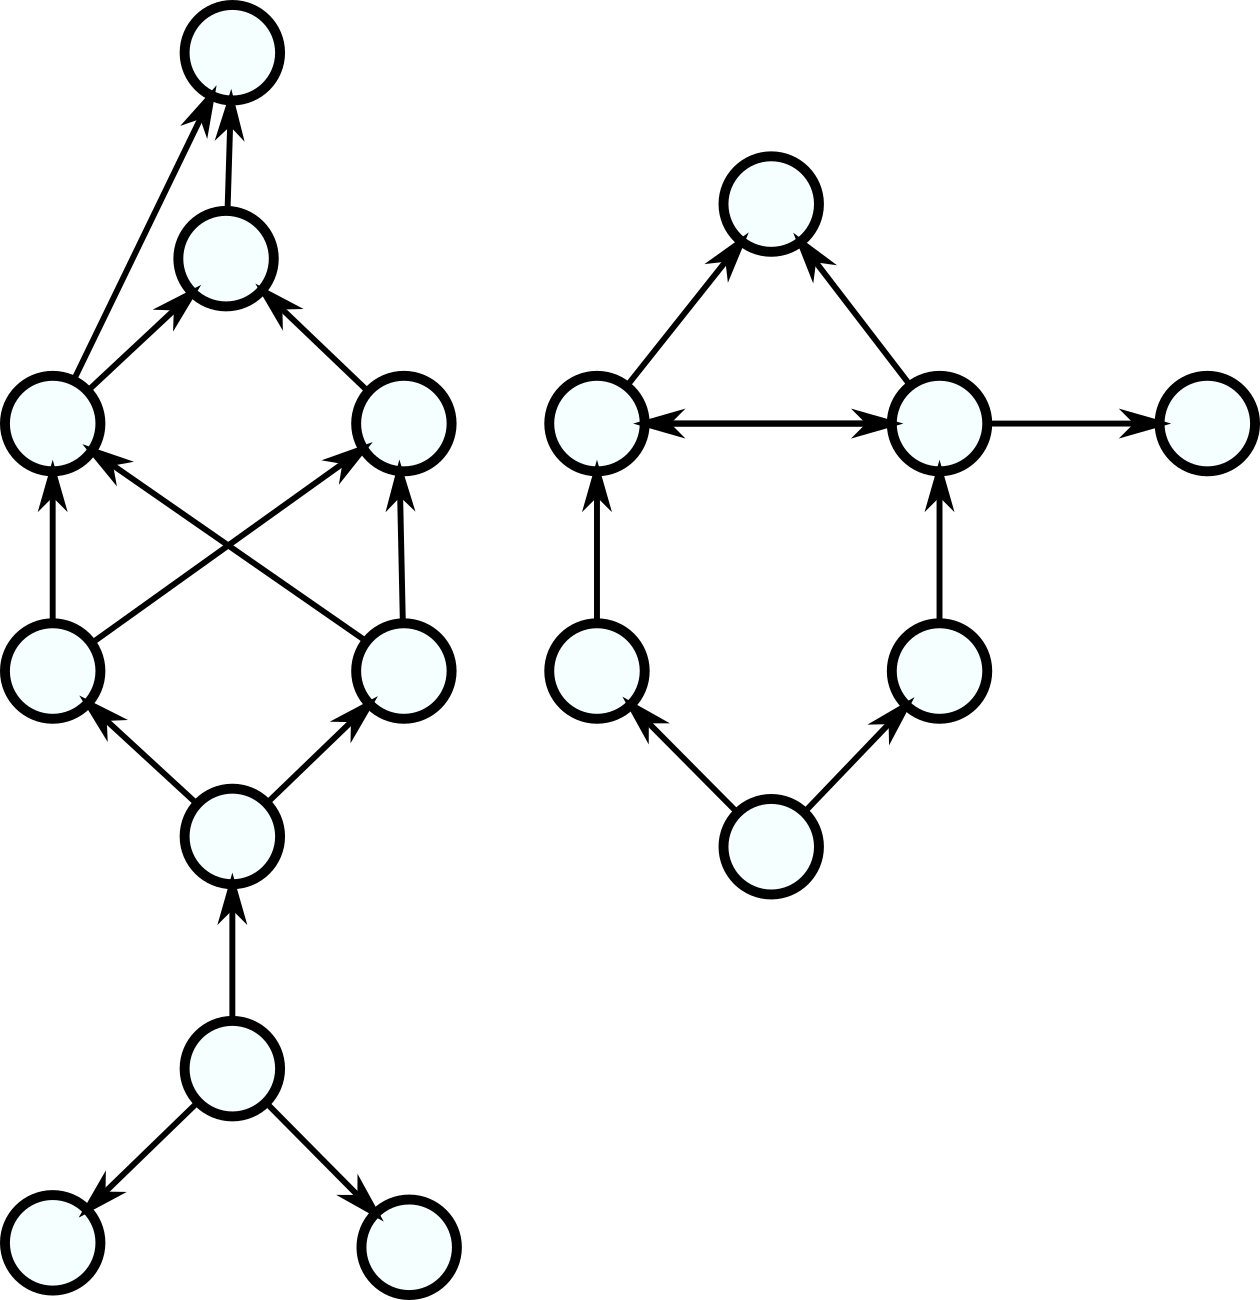
\includegraphics[scale=0.3]{Figures/result1.png}}}
	\qquad
	\subfloat[]{{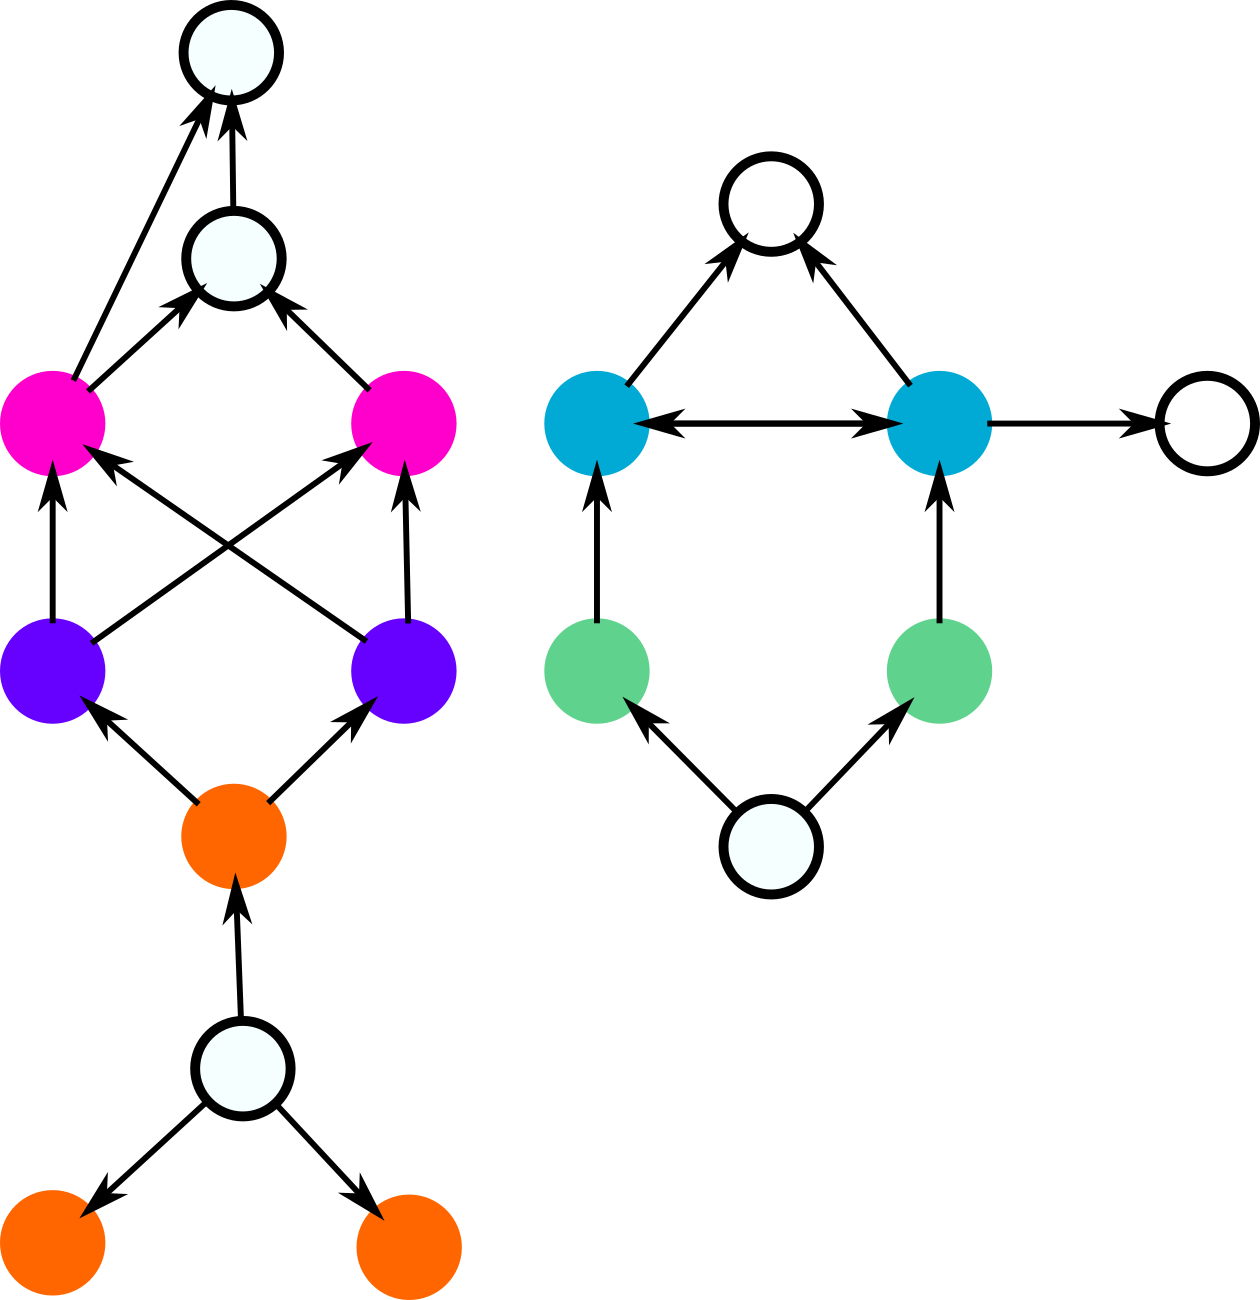
\includegraphics[scale=0.3]{Figures/result1-1.png}}}
	\caption{First trial network example. Containing a total of $N = 17$ nodes and $M = 22$ arcs, the network has two weakly connected components, defined as the connected networks when we treat all the directed arcs as undirected edges. For each non-trivial fiber I give the same color for the nodes belonging to it.}
	\label{fig:result1}
\end{figure}

At the end of the algorithm, all the identified fibers are input-tree stable with respect to all fibers in the network, including the fiber itself. Then, by labelling each fiber with an index or color we can then construct the fibration building blocks through the calculation of the fundamental class number $n$ and through the subclass number $\ell$. Again, a fibration building block is defined as the nodes belonging to a fiber and all the $\ell$ external nodes that directly regulates at least one node of the current fiber. With that, we calculate the fundamental class number $n_k$ of the fiber $k$ by building the adjacency matrix $\mathbf{A}^{k}$ of its fibration building block and then calculating the largest eigenvalue of it. The value of $n$ quantifies the information cycles of the fibration building blocks and it can be either represent integer branching ratios or fractal golden ration of their input-tree topology class.

Labelling the resulted fiber distribution for the first example in figure \ref{fig:result1}, we obtain the following fibration classification for each fibration building block of the network containing more than one node:

\begin{figure}[!ht]
    \centering
    \subfloat[]{{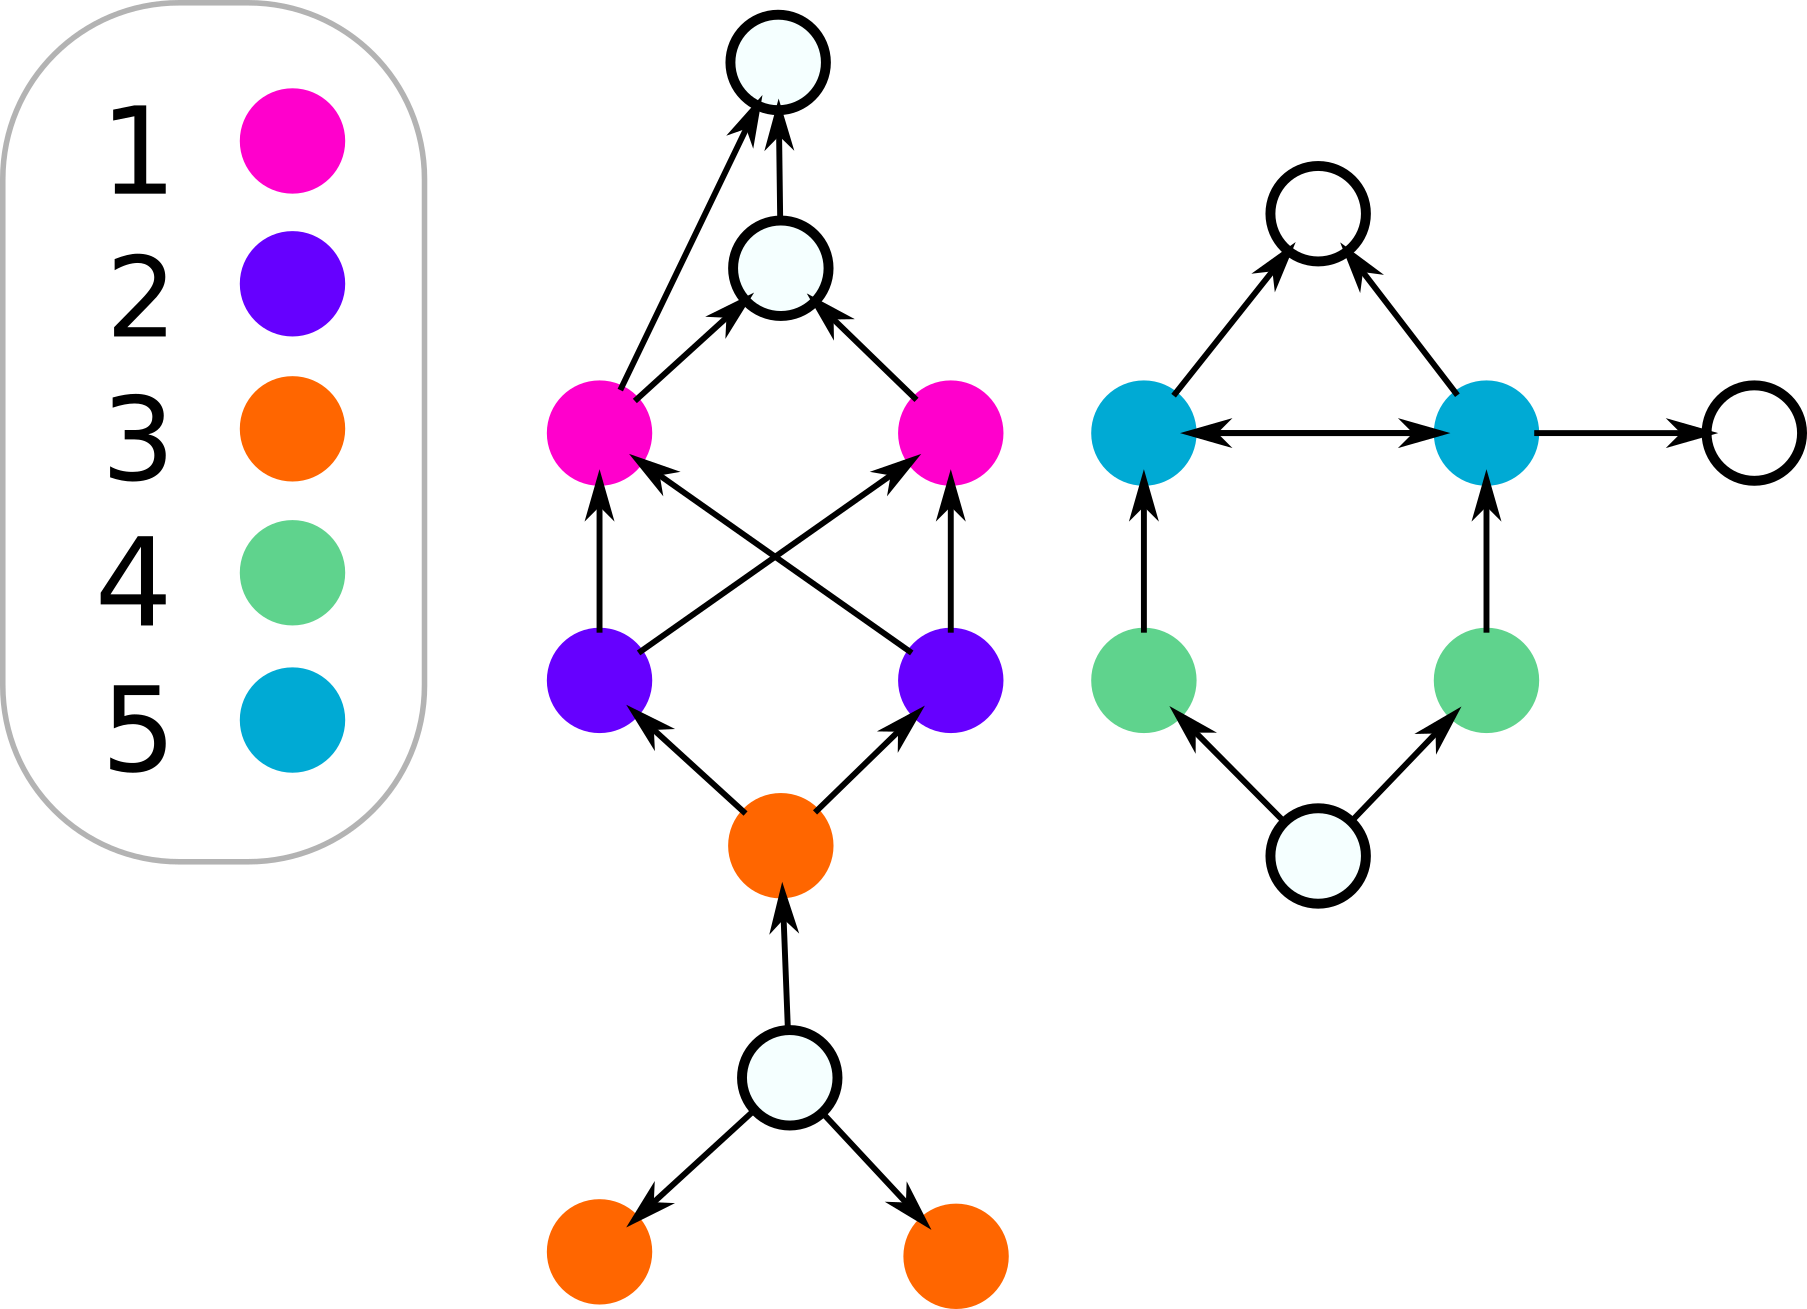
\includegraphics[scale=0.22]{Figures/result1-label.png}}}
    \qquad
    \begin{tabular}[b]{cc}\hline
      Fiber & $| n, \ell \rangle$  \\ \hline
      1 & $| 0, 2 \rangle$ \\
      2 & $| 0, 1 \rangle$ \\
      3 & $| 0, 1 \rangle$ \\ 
      4 & $| 0, 1 \rangle$ \\
      5 & $| 0, 2 \rangle$ \\ \hline
	\end{tabular}
	\captionlistentry[table]{A table beside a figure}
    %\captionsetup{labelformat=andtable}
    \caption{A table beside a figure}
\end{figure}

The second example exhibits a connected component containing $N = 21$ nodes, where all the three type of regulation are present. For this network I find the total of eleven fibers, where only six are fibers containing more than one node in it. Important to note that for two arbitrary nodes be in the same fiber they must not just receive the same number of inward connections but the same number of each type of inward connections, receiving, this way, equivalent information from the rest of the network. We can see this for the example of the fibers $4$ e $5$, where even though both receives two links from the same central node, the fibers receives different types of information from that node, meaning that they are not equivalent fibers.

If we consider the fiber $3$, besides the inner autoregulation loop we have a loop information going outside the fiber and going back through an external regulator inside the fiber $1$. In cases like this the branching ratio of the fiber has a fractal value given by a golden branch ratio $\phi_d$ resulted by a cycle of information represented by a fibonacci sequence. This way, fiber $3$ can be classified by the values $| \phi_d, \ell = 2 \rangle$ where the fiber has two external regulator nodes. The fibration classification for the non-trivial fibers is showed in the table \ref{tab:r2}.

%\begin{figure}[H]
%	\centering
%	\subfloat[]{{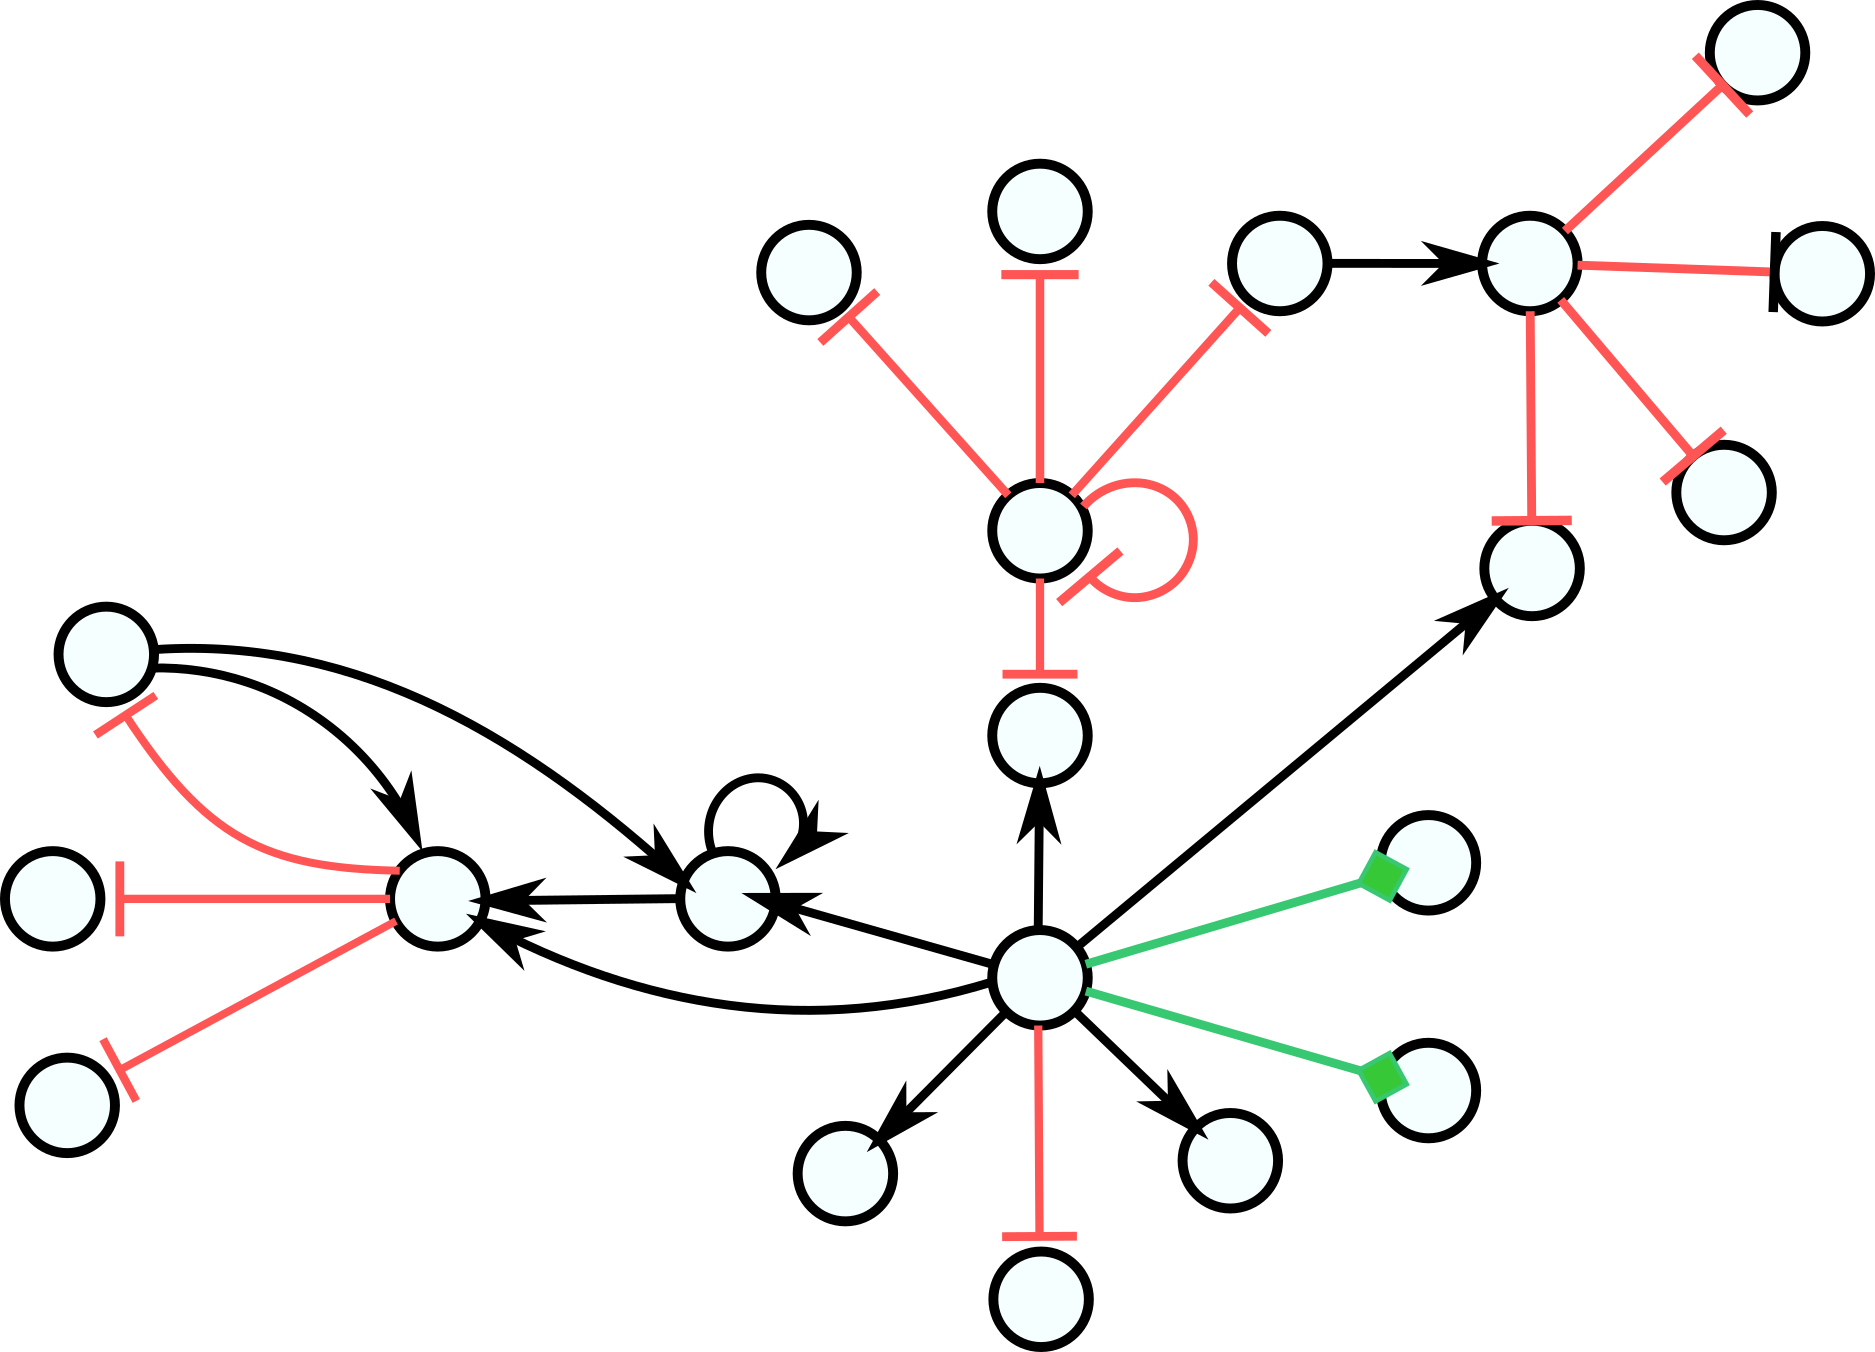
\includegraphics[scale=0.25]{Figures/result2.png}}}
%	\qquad
%	\subfloat[]{{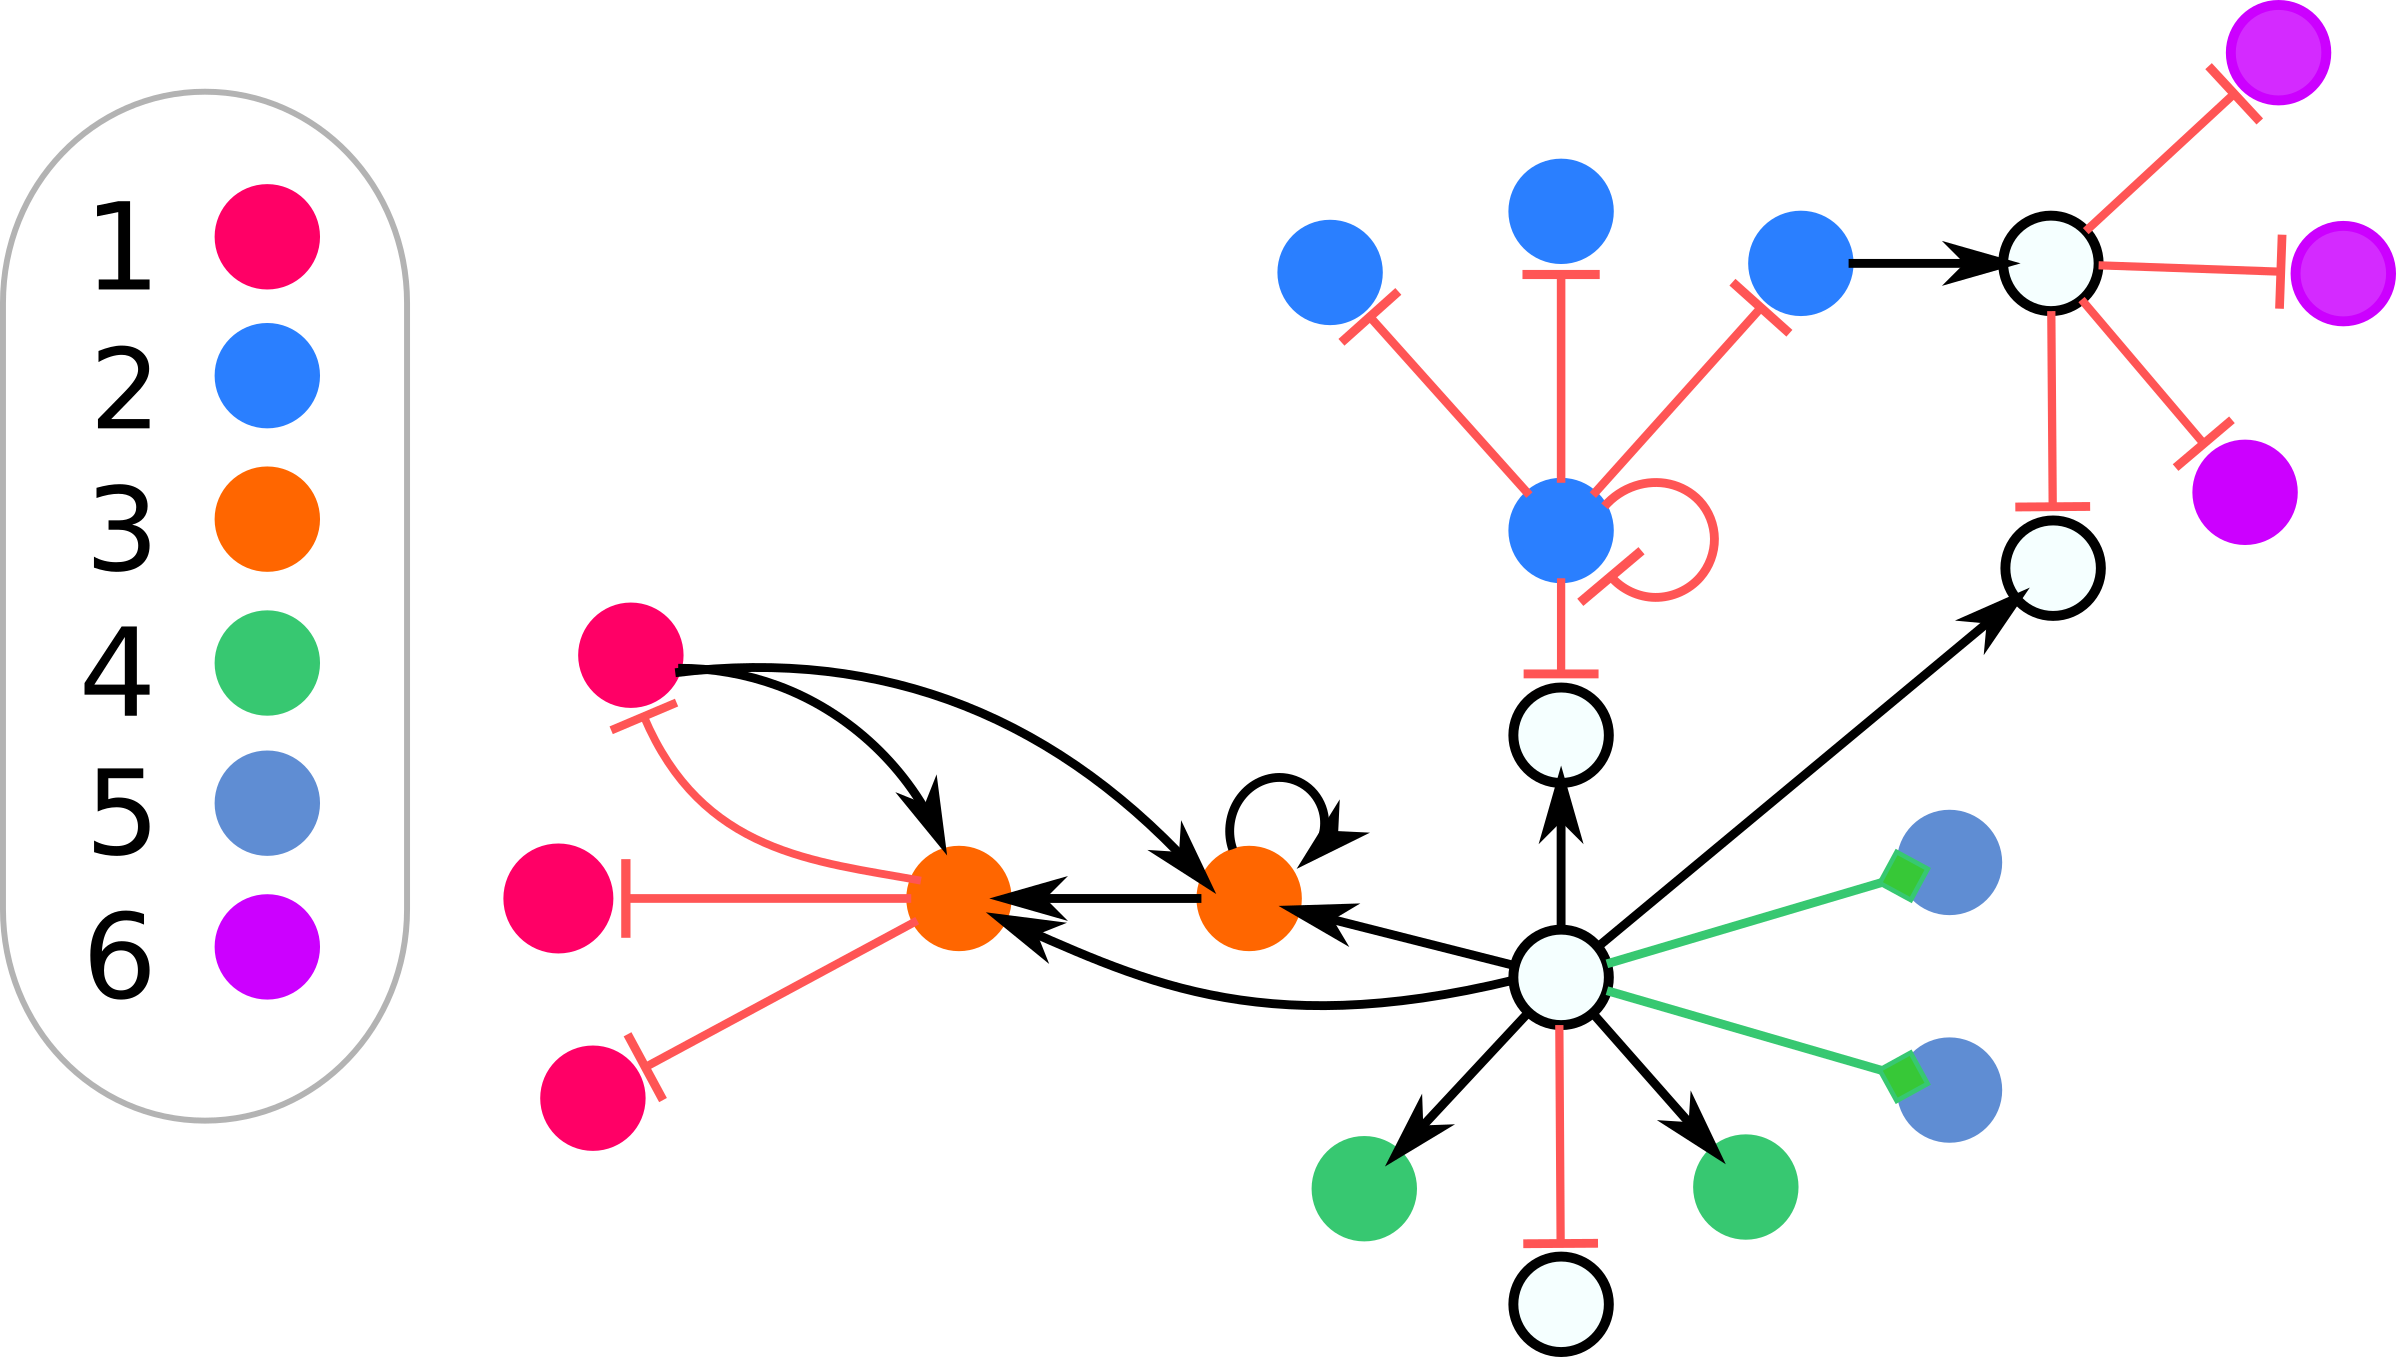
\includegraphics[scale=0.25]{Figures/result2-label.png}}}
%	\caption{First trial network example. Containing a total of $N = 17$ nodes and $M = 22$ arcs, the network has two weakly connected %components, defined as the connected networks when we treat all the directed arcs as undirected edges. For each non-trivial fiber I %give the same color for the nodes belonging to it.}
%	\label{fig:result2}
%\end{figure}

\begin{figure}[H]
	\centering
	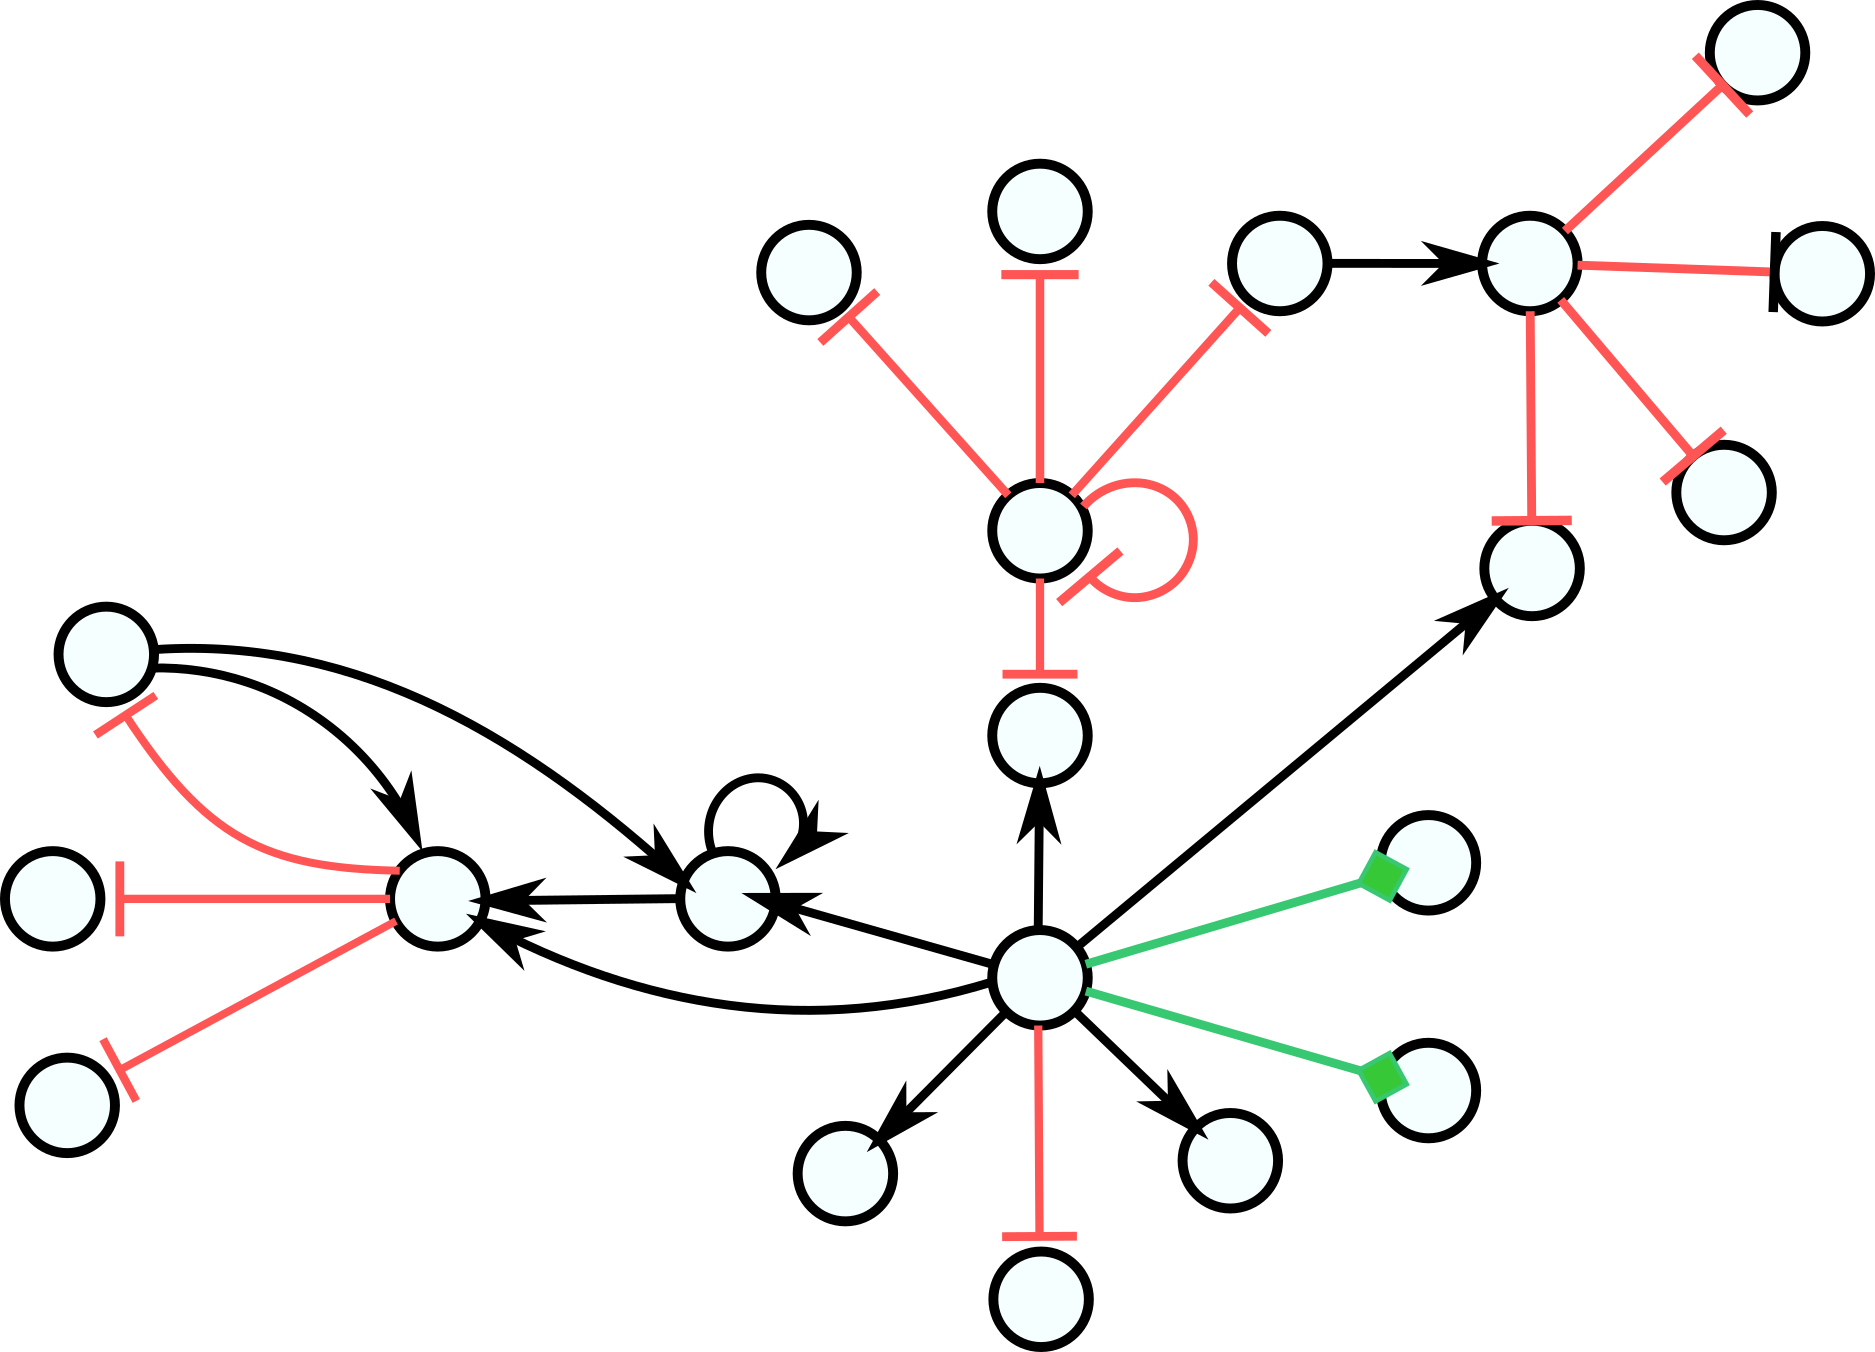
\includegraphics[scale=0.275]{Figures/result2.png}
\end{figure}

\begin{figure}[H]
	\centering
	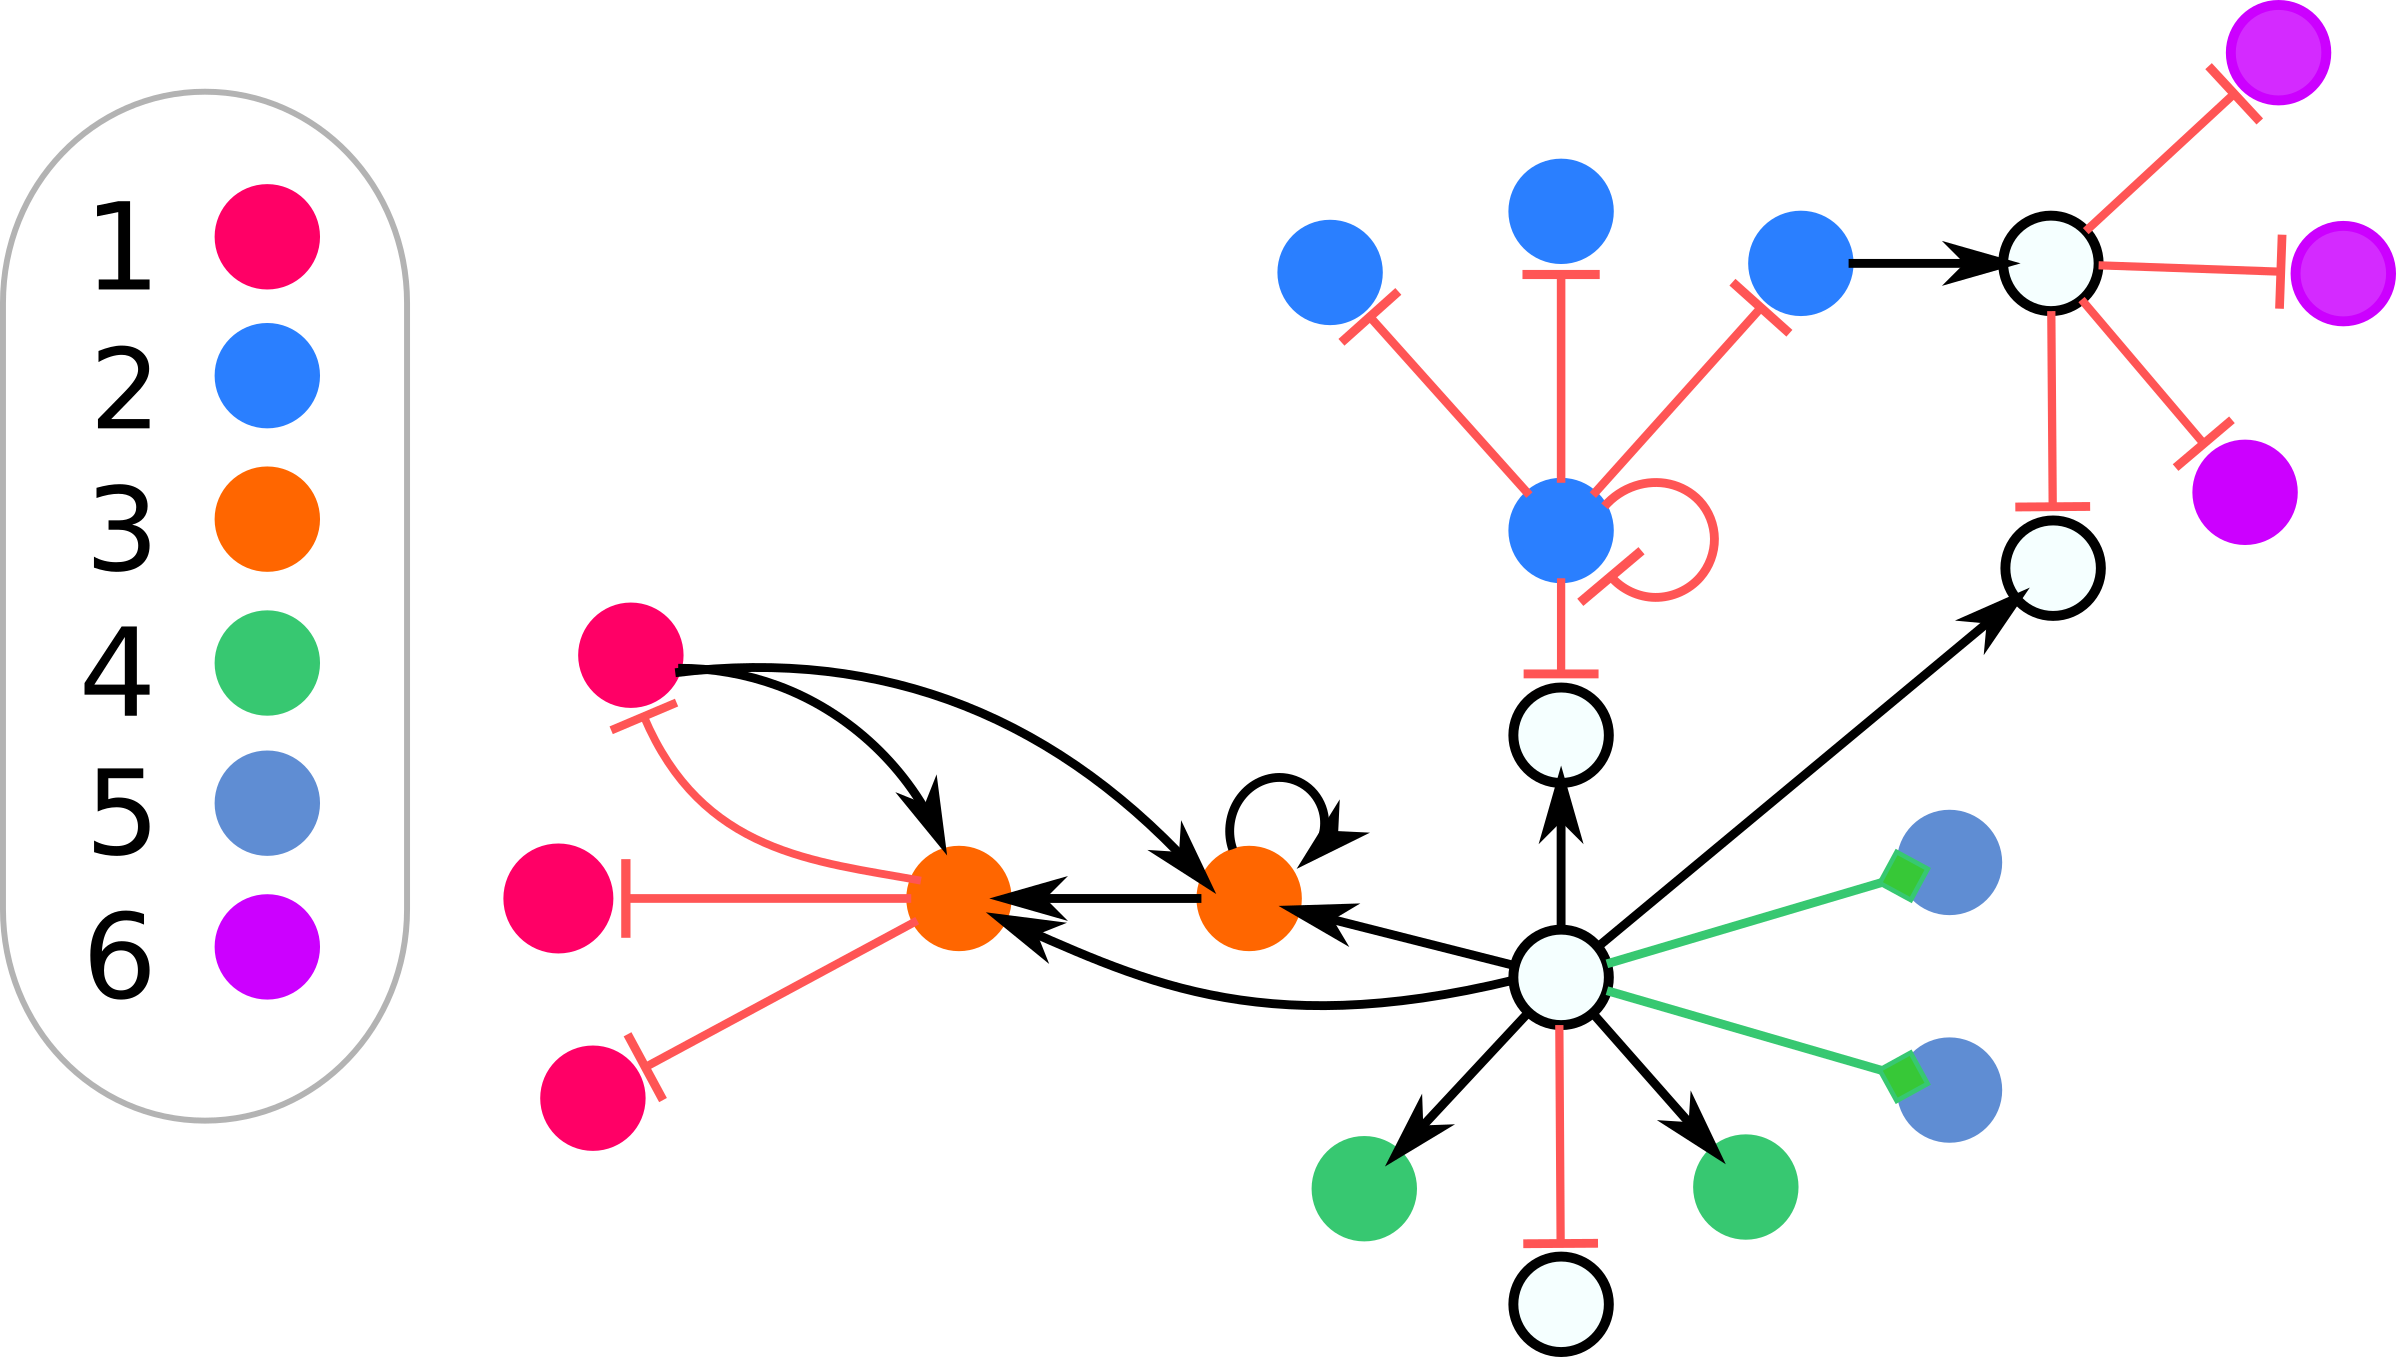
\includegraphics[scale=0.275]{Figures/result2-label.png}
\end{figure}

\begin{table}[H]
\centering
\begin{tabular}[b]{cc}\hline
	Fiber & $| n, \ell \rangle$  \\ \hline
	1 & $| 0, 1 \rangle$ \\
	2 & $| 0, 1 \rangle$ \\
	3 & $| 0, 1 \rangle$ \\ 
	4 & $| 0, 1 \rangle$ \\
	5 & $| 0, 2 \rangle$ \\
	6 & $| 0, 2 \rangle$ \\ \hline
  \end{tabular}
  \caption{}
  \label{tab:r2}
\end{table}

Before applying the algorithm for the whole \textit{Escherichia Coli} network, I chose, for the finality of visualization and testing, to apply first the algorithm for a weakly connected component of the \textit{E. Coli} network. The same network is showed at the supplementary information of \cite{fibration2019}. The fiber distribution found is consistent with the one presented at \cite{fibration2019}, presenting the total of fifteen non-trivial fiber groups as shown in the figure \ref{fig:result3-1}.

\begin{figure}[H]
	\centering
	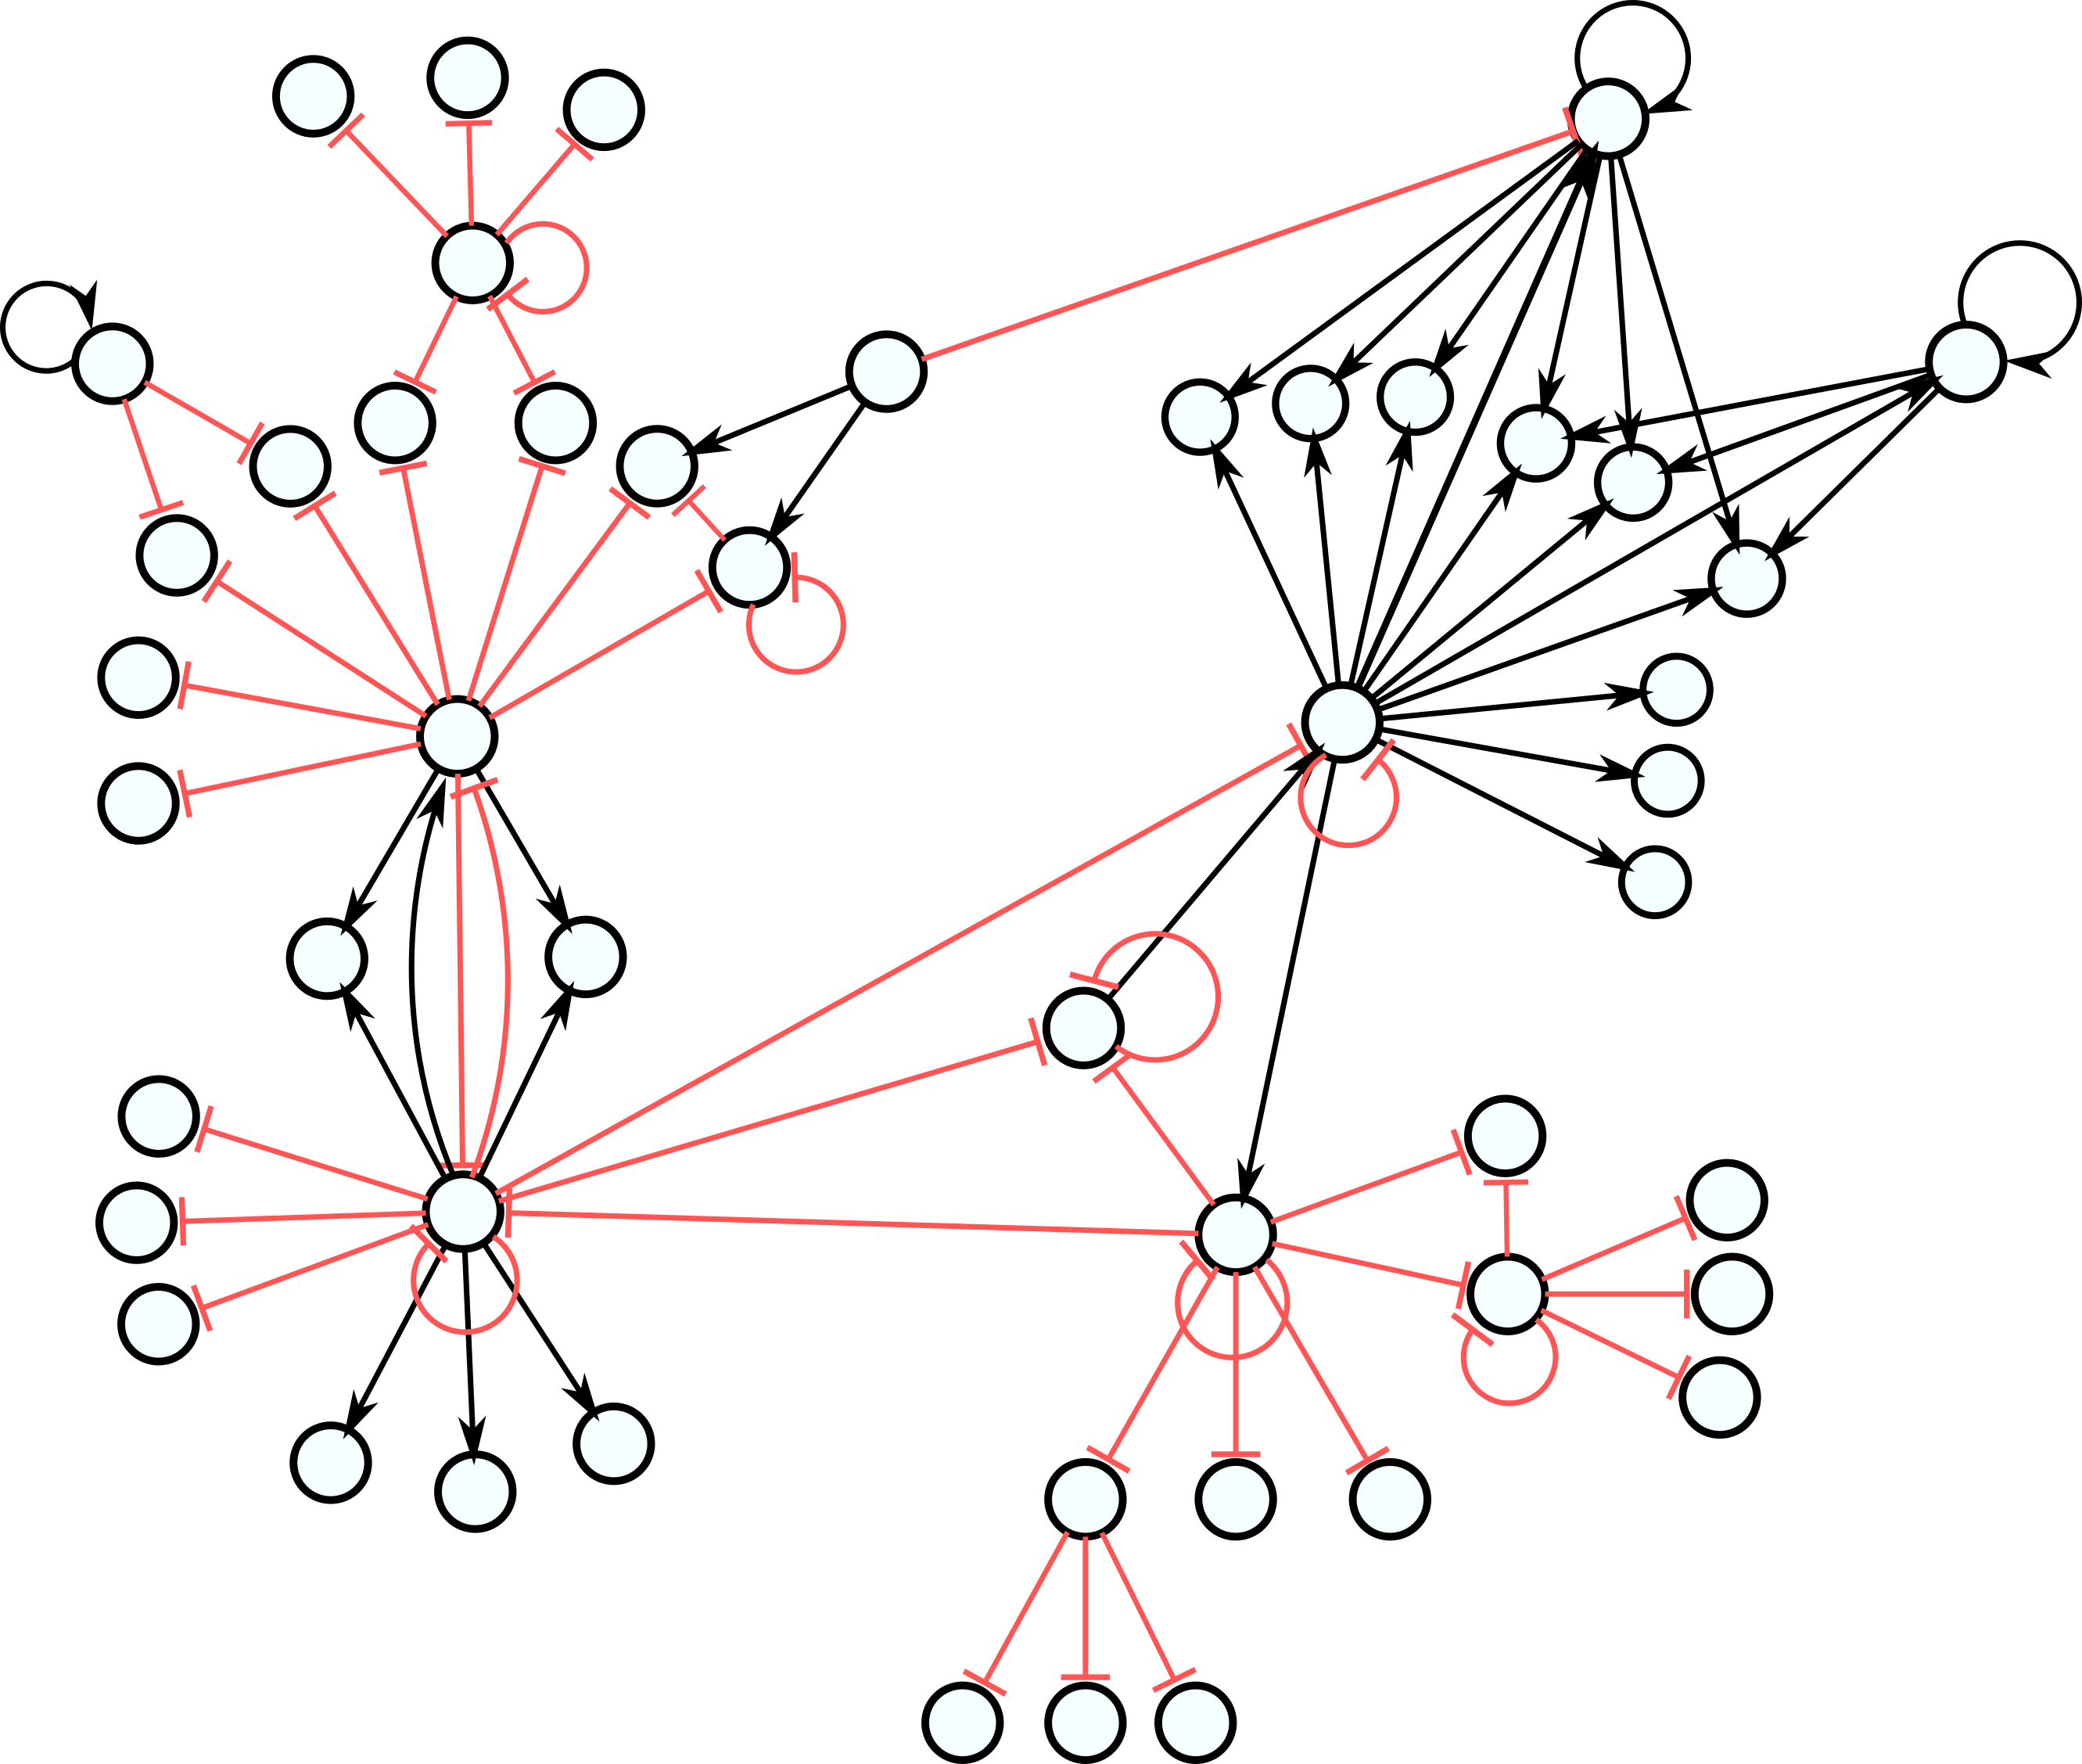
\includegraphics[scale=0.27]{Figures/result3.png}
	\caption{}
	\label{fig:result3}
\end{figure}
\begin{figure}[H]
	\centering
	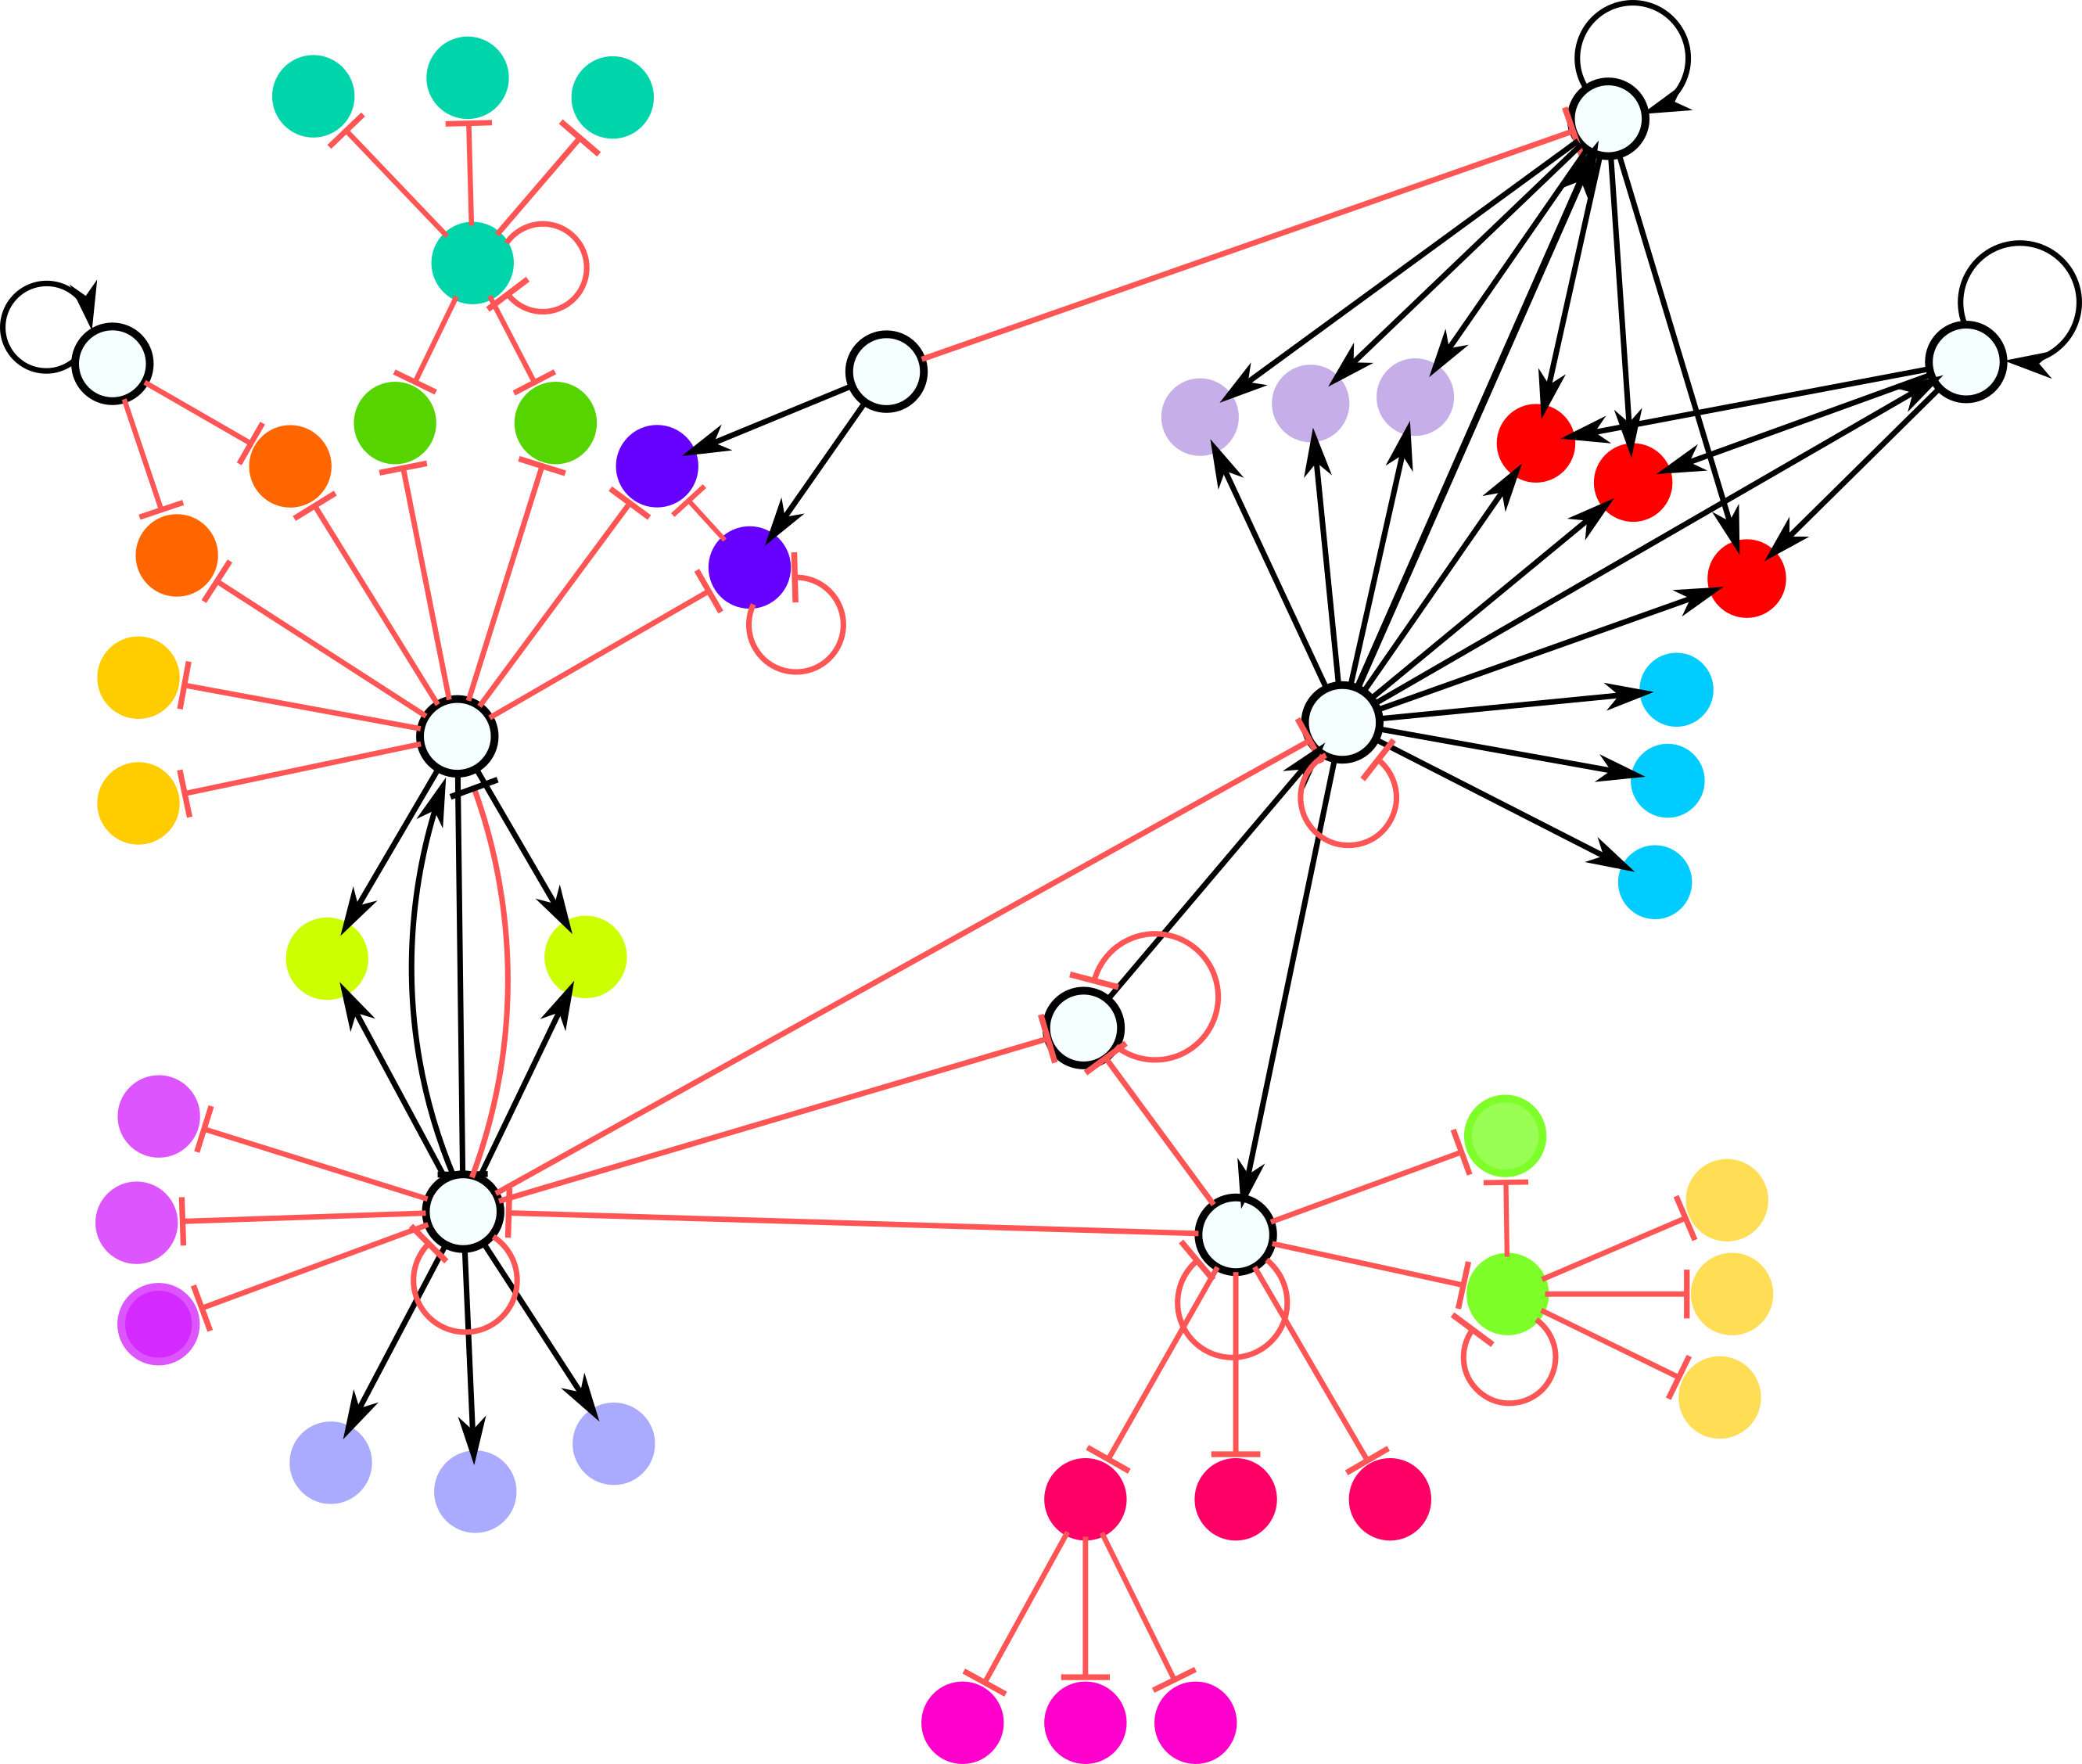
\includegraphics[scale=0.27]{Figures/result3-1.png}
	\caption{}
	\label{fig:result3-1}
\end{figure}

The connected component showed at the figure \ref{fig:result3} is a subset representation of the nodes of the regulatory network of the \textit{Escherichia Coli} bacteria and the resulted fibers shows just a portion of the whole fibers pattern. In the table X I provide the classification for each fibration building block obtained for the whole bacteria network, including, of course, the fibers presented in the figure \ref{fig:result3-1}. In total, I have found $92$ non-trivial fiber groups containing a total of $416$ nodes, obtaining a characteristic fiber statistics for the \textit{Escherichia Coli} network data. To guarantee the correctness of the fiber distribution found I calculated, after the refinement algorithm, the information received for each node inside the fibers and compares if each one process equivalent information. The result of this calculation is stored in the data file given at \url{https://github.com/higorsmonteiro/fiberblocks/blob/master/Data/fiberVerification.dat}, where for each node in a non-trivial fiber block I give the list of the nodes that sends information messages to the current node along with their fiber indexes and type of link values. Thus, the results of this report show an equivalent fiber distribution over the network comparing with results exhibited at \cite{fibration2019} for the same regulatory network data. After the classification for each fiber is done, I notice that the $92$ fibers are reduced by one unit, because of the existence of a multilayered fiber compound by two fibers. This way, the number of fibers are consistent with \cite{fibration2019}.

The statistics concerning the fundamental class number and the external regulators of each fibration block on the network is given in the table X, showing \textcolor{red}{describe the pattern of the statistics of the table that concerns the bacteria fiber statistics}.


%----------------------------------------------------------------------------------------
%	BIBLIOGRAPHY
%----------------------------------------------------------------------------------------

\bibliographystyle{unsrt}

\bibliography{sample.bib}

%----------------------------------------------------------------------------------------

\end{document}
